\documentclass[10pt,a4paper,cleardoubleempty]{scrbook}


\usepackage{natbib}
\usepackage[italian]{babel}
\usepackage{classicthesis-ldpkg}
\usepackage[parts,linedheaders,pdfspacing,subfig,
  eulerchapternumbers,eulermath,dottedtoc,listings]{classicthesis}
\usepackage{lipsum}
\usepackage{epigraph}
\usepackage[T1]{fontenc}
\usepackage[utf8]{inputenc}
\usepackage{graphicx}
\usepackage{gensymb}
\usepackage{amssymb}
\usepackage{amsmath}
\usepackage{booktabs}
\usepackage{multirow}
\usepackage{array}


\hyphenation{back-end front-end SapWin SapecNG Sapec QSapecNG}

\newcolumntype{i}{>{\centering\arraybackslash} m{.25\linewidth} }

\lstdefinelanguage{pseudocode}
  { morekeywords={se, allora, altrimenti, procedura, inizio, fine} }


\areaset[5mm]{312pt}{699pt}

\title{\begin{huge}\bfseries QSapecNG\end{huge}}
\author{Michele Caini}



\begin{document}

\thispagestyle{empty}

\begin{center}
  \begin{center}
    
\includegraphics[scale=0.75]{immagini/salomone.pdf}
  \end{center}
  Università degli Studi di Firenze\\
  Facoltà di Ingegneria\\
  \rule{9cm}{0.5mm}\\[0.3cm]
  Corso di Laurea Specialistica in\\ Ingegneria Informatica\\
  \vspace{3cm}
  {
    \begin{Large}\textbf{Il Simulatore Circuitale}\end{Large}\\\vspace{10pt}
    \begin{huge}\textbf{QSapecNG}\end{huge}\\\vspace{10pt}
    \begin{large}Qt-based Symbolic Analysis Program for Electric Circuits\end{large}\\\vspace{10pt}
    \begin{large}New Generation\end{large}
  }\\
  \vspace{2.5cm} { 
\includegraphics[scale=0.45]{immagini/qsapecng.pdf} }\\
  \vspace{\stretch{1}}
  \begin{normalsize}
    \textbf{Relatore:}\hspace{10pt}Luchetta Antonio\hspace{\stretch{1}}\vspace{5pt}\\
    \textbf{Relatore:}\hspace{10pt}Manetti Stefano\hspace{\stretch{1}}\vspace{5pt}\\
    \textbf{Candidato:}\hspace{10pt}Caini Michele\hspace{\stretch{1}}\vspace{5pt}\\
  \end{normalsize}
  \vspace{1.5cm}
  \hspace{\stretch{1}} A.A. 2009/2010
\end{center}


\cleardoublepage
\null\vspace{\stretch{1}}\begin{flushright}
\setlength{\epigraphwidth}{21em}
\epigraph{
Ardo dal desiderio di spiegare, e la mia massima soddisfazione è prendere qualcosa di ragionevolmente intricato e renderlo chiaro passo dopo passo.\\
È il modo più facile per chiarire le cose a me stesso.
}{Civiltà extraterrestri\\ Isaac Asimov}
\end{flushright}\vspace{\stretch{2}}\null

\cleardoublepage
\tableofcontents


\cleardoublepage
\part{Introduzione}

\thispagestyle{empty}
\null\vspace{\stretch{1}}
\begin{flushright}
\setlength{\epigraphwidth}{21em}
\epigraph{
\footnotesize{``Mi avete detto qual'è la prima regola della saggezza'' dissi. ''E la seconda, quale sarebbe ? ``\\
''A questo si può rispondere'' disse. ''Ce ne sono cinque in tutto. Fa tutte le domande che devi fare e non rispondere mai a nessuna. Volgi tutto quello che senti a tuo vantaggio. Portati sempre dietro il necessario per le riparazioni. Svolta a sinistra ogni volta che puoi. Non adoperare mai per primo il freno davanti``.\\
''Sono regole interessanti`` dissi asciutto.}
}{\footnotesize{Il terzo poliziotto\\ Flann O'Brien}}
\end{flushright}\vspace{\stretch{2}}\null

\chapter{Metodi di Risoluzione Simbolica}

\section{Motivazioni}

L'analisi simbolica di circuiti elettrici rappresenta una tecnica formale per lo studio di questi ultimi, fornendo un'ampia gamma di informazioni utili sulle diverse caratteristiche del circuito stesso. Tale tecnica ha visto negli anni l'alternarsi di periodi di fervida attenzione a momenti di blanda considerazione, prevalentemente a causa della complessità computazionale che, col passare del tempo, è diventata uno scoglio sormontabile data la crescente potenza di calcolo a disposizione, riportando in auge l'argomento.\\
L'analisi simbolica può essere usata per lo studio di comportamenti specifici o caratteristiche legate alle variabili dipendenti, le variabili indipendenti e a tutti gli altri elementi che concorrono a comporre un circuito. A differenza e in aggiunta a ciò che si propone di fare l'analisi numerica (che oltre ad offrire migliori prestazioni in termini prettamente computazionali, permette di ispezionare il comportamento di un circuito sotto svariati aspetti), l'approccio simbolico aiuta lo sviluppatore a comprendere meglio quali elementi incidano effettivamente, in modo più o meno significativo, su tale comportamento. Da notare che, sebbene ad oggi lo studio simbolico sia limitato ad un ben definito insieme di elementi, è possibile avvicinare anche oggetti altrimenti al di fuori dalla portata dello strumento attraverso approssimazioni note nell'ambito elettronico. A supporto di questa tesi, si possono considerare ad esempio le approssimazioni per piccoli segnali e il modello di Giacoletto (per le alte frequenze) utili all'approssimazione di transistor a giunzione.

\begin{figure}[hb]
 \centering
 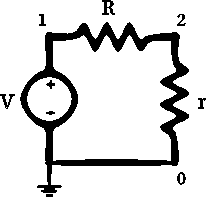
\includegraphics{immagini/vdiv.pdf}
 \caption{Partitore di tensione}
 \label{fig:vdiv}
\end{figure}

Nonostante la complessità degli algoritmi sviluppati negli anni, tale metodologia offre la possibilità di un'analisi veramente flessibile ed esclusiva, riservata ai soli componenti di interesse. Dall'analisi simbolica si possono infatti ricavare diverse forme di espressione per le variabili d'interesse di un circuito. Si consideri a tal proposito il semplice partitore di tensione in figura \ref{fig:vdiv}, supponendo di voler attribuire una rappresentazione simbolica al generatore di tensione $V$ e alla resistenza $R$, trattando invece la resistenza $r$ come valore numerico, poiché in essa non è riposto alcun interesse. Poniamo inoltre che il generatore abbia come valore numerico 3 V, la prima resistenza 5 \ohm\ e la seconda resistenza 1 \ohm.\\
Otteniamo attraverso la risoluzione simbolica, banalmente, tre forme anziché una per la funzione di trasferimento.\\
Più nello specifico avremo una forma puramente simbolica, ovvero: $$ \frac{V * r}{R + r} $$
Una forma ricavata sostituendo ad ogni elemento la sua rappresentazione numerica, come segue: $$ \frac{3 * 1}{1 + 5} = \frac{1}{2} $$
Infine una forma mista che, una volta compressa e semplificata (minimizzandola e rendendola più comprensibile all'essere umano), meglio rappresenta e si plasma sulla base delle intenzioni dell'utente: $$ \frac{V * 1}{R + 1} = \frac{V}{R + 1} $$

La forma mista sintetizza, di fatto, il comportamento del circuito mettendo in evidenza le sole variabili di interesse e trattando come numeriche, attraverso opportune sostituzioni, tutte le altre. Risulta importante sottolineare l'accenno fatto sopra alle operazioni di compressione e semplificazione. Uno dei rischi in cui si incorre è, infatti, quello di ricavare da tali procedure formule di dimensioni notevoli e difficili da interpretare. Tali formule, attraverso opportune riduzioni, risulterebbero di gran lunga più facilmente gestibili. Pertanto i passi di semplificazione delle espressioni non vanno trascurati poiché anch'essi molto importanti nella catena di sviluppo del risultato.

\paragraph{}
Un altro aspetto da non tralasciare, che non traspare da quanto introdotto finora, è dato dalla possibilità di portare avanti operazioni di analisi numerica sulle formule ottenute. Può sembrare scontato ma la sola osservazione della forma mista richiesta può dare indicazioni all'utente su chi influenza il comportamento del circuito senza esplicarne il come. Del resto anche questa è una informazione interessante e l'analisi simbolica ci viene incontro fornendo la possibilità di ottenere curve di ogni genere al variare dei parametri, così da ricercare quella che meglio approssima il comportamento desiderato. Gestendo infatti formule miste si può procedere banalmente alla sostituzione progressiva di valori associati ai componenti, con l'analisi in determinati intervalli di frequenze e così via.\\
Nulla vieta, in effetti, di effettuare con una forma mista o simbolica tutte o gran parte di quelle operazioni che si possono svolgere di norma con un risolutore numerico.

\paragraph{}
Riassumendo, quindi, è possibile trovare nell'uso di risolutori simbolici (anziché numerici) una maggiore flessibilità per quanto riguarda l'approccio e lo studio del problema, avendo la possibilità di sondarlo da diversi punti di osservazione. Di contro, però, non va trascurata la maggiore richiesta computazionale per questo tipo di analisi che, pertanto, va usata laddove vi sia veramente bisogno.\\
Un approccio plausibile potrebbe essere quello di un'analisi a più fasi durante le quali, in base alle necessità e ai problemi che si propongono, si affronta lo studio attraverso risolutori prettamente simbolici o prettamente numerici. Sconsigliato l'uso di un risolutore simbolico in ambiti dove vi sia la necessità della sola analisi numerica e, viceversa, l'uso di risolutori numerici non è possibile se si hanno richieste di analisi simbolica.

\paragraph{}
Molto importante è capire che i due strumenti, risolutori simbolici e numerici, non sono alternativi ma complementari ed entrambi arricchiscono il parco di oggetti che un progettista può avere a disposizione per assolvere al suo compito.


\section{Cenni storici}

Le metodologie di analisi numerica si sono evolute negli anni, migrando addirittura da un ambito prevalentemente matematico (dove si procedeva con operazioni matriciali) allo spazio dei grafi. In quest'ultimo ambito, in particolare grazie ai contributi ottenuti prima da Grimbleby \cite{Grimbleby} e quindi da Schach \cite{MRT}, sono state notevolmente abbattute le barriere di complessità computazionale, aspetto che, in concomitanza alla sempre crescente potenza di calcolo a disposizione, ha permesso lo sviluppo di nuovi e performanti algoritmi, tutt'oggi in uso.

L'analisi simbolica dei circuiti elettrici tiene banco nell'ambiente elettronico fin dagli anni '70, poiché risultano innegabili i vantaggi che essa può portare se affiancata all'analisi numerica. Del resto, come già anticipato, fin dagli albori ha trovato estimatori nell'ambito teorico e critici nell'ambito pratico, risultando praticamente inattuabile se non a circuiti dalle dimensioni estremamente limitate e per i quali, di fatto, non risultasse realmente necessaria.

Le metodologie di risoluzione proposte hanno trovato terreno fertile prevalentemente in due aree tematiche, rendendosi note attraverso i \textit{metodi algebrici} e i \textit{metodi topologici}.

Senza addentrarsi nello specifico, la prima categoria ricavava le formule desiderate attraverso tecniche di manipolazione simbolica delle espressioni algebriche applicate alle equazioni della rete. Ciò richiedeva al contempo un grosso impegno computazionale e grandi quantitativi di memoria, tanto per la memorizzazione quanto per l'elaborazione. I metodi algebrici hanno quindi ceduto il passo ai metodi topologici. Questi ultimi hanno permesso di snellire i processi di risoluzione (guadagnando in termini di risorse di calcolo), per la memorizzazione e per l'espletamento delle proprie funzioni. Uno dei primi esempi applicabili in tal senso è citato in \cite{Grimbleby} e sviluppato in \textit{Sapec}\graffito{Sapec (Symbolic Analysis Program for Electric Circuits) è un risolutore simbolico privo di interfaccia grafica, che riceve dati in ingresso come parametri da riga di comando}, cuore del software \textit{SapWin}\graffito{SapWin (Symbolic Analysis Program for Windows) è un'interfaccia sviluppata per ed intorno a Sapec ed invoca quest'ultimo nelle fasi di risoluzione} ed entrambi predecessori di \textit{QSapecNG}, il quale implementa invece al suo interno un'evoluzione dell'algoritmo di cui sopra, come proposta in \cite{MRT}. Scendendo un po' più nel dettaglio dei metodi topologici, bisogna osservare che un attento studio delle strutture dati, delle relazioni fra esse e dei metodi di accesso alle informazioni può portare a notevoli migliorie sotto ogni aspetto. Anche per questo tali metodologie hanno trovato largo consenso e suscitato l'interesse di studiosi tuttora intenti a perfezionarne il comportamento. Basti pensare infatti che, sotto determinate condizioni, i metodi topologici si riducono ad algoritmi su grafi pesati (che rappresentino opportunamente il circuito in esame). A tali grafi e algoritmi possono pertanto essere applicate tutte le tecniche di compressione e ottimizzazione conosciute, guadagnando ulteriormente in prestazioni.

\paragraph{}
Da quanto brevemente detto si intuisce come sia vivo e vitale il mondo intorno a questa categoria di problemi, anche a causa dell'importanza non relegata esclusivamente all'ambito accademico ma estesa anche a quello commerciale. Purtroppo, però, la complessità del problema affrontato è tale da rendere difficoltoso il cammino e difficile il processo evolutivo degli algoritmi coinvolti.


\section{Da Sapec a QSapecNG, attraverso SapWin}

Per quanto riguarda la storia legata al software qui discusso, esso nasce, cresce e si sviluppa interamente all'interno dell'Università degli Studi di Firenze. \textit{SapWin} si appoggia sul motore di analisi \textit{Sapec}, un software separato dall'interfaccia grafica per scelta degli sviluppatori e attraverso l'uso di quest'ultimo arriva fino all'attuale versione 3.0, ampliando il suo parco di funzionalità ma senza sostituire l'algoritmo che fa da base al processo di risoluzione. Eppure tanto SapWin quanto Sapec rappresentano il frutto di anni di studi teorici e implementazioni pratiche dei loro padri.\\
Una discussione sul mondo di SapWin esula però da questo lavoro e richiederebbe svariati capitoli per poter sciogliere tutti i nodi.

Nel suo piccolo, invece, \textit{QSapecNG} nasce come il frutto di un lavoro iniziato durante il percorso di studi triennale dell'autore, conclusosi in una prima fase con lo sviluppo di SapecNG. Quest'ultimo era costituito da un motore di risoluzione scritto in C e un semplice parser LALR (\textit{LookAhead Left to Right parser}) basato su \textit{flex/bison}\graffito{Flex (Fast Lexical Analyzer) e Bison (GNU Parser Generator) sono una coppia consolidata nel mondo dei compiler-compiler o generatori di compilatori}, era in grado di elaborare i file prodotti in forma di \textit{netlist} da SapWin e quindi catturare le informazioni richieste restituendole all'utente. La peculiarità di SapecNG non risiedeva però tanto in funzionalità particolari messe a disposizione, strumenti innovativi utilizzati od ottimizzazioni di alcun genere, bensì nello sviluppo di un algoritmo che migliorasse le prestazioni di Sapec: da questo la decisione della dicitura \textit{NG}, o \textit{Next Generation}, a simboleggiare il passo avanti in termini di evoluzione fatto nell'ambito del progetto in seno all'Università di Firenze. Altra caratteristica importante e mantenuta nel tempo era la sua portabilità, ad oggi e sempre più un aspetto necessario per programmi di nuova generazione. La carenza principale di SapecNG risiedeva nella possibilità di utilizzo da sola riga di comando e nella troppa rigidità del codice, il che rendeva il software utile al solo scopo didattico.

Con QSapecNG vi è stata una riscrittura per intero del software SapecNG, migrando il codice da C a C++ e sfruttando le potenzialità offerte da librerie esterne quali \textit{Boost C++} \cite{BGL} e il framework \textit{Qt} \cite{Qt}. L'attenzione al design ha mantenuto una netta separazione fra backend e frontend, così da permettere in futuro la riscrittura di una GUI anche attraverso diverse librerie e al contempo dando la possibilità di evolvere il motore sottostante e le funzionalità offerte senza incidere in maniera significativa o difficilmente gestibile sull'interfaccia utente. Le tecniche di sviluppo del software e i pattern più o meno noti applicati, hanno permesso di rendere elegantemente complicati alcuni frangenti altrimenti ostici. Infine, anche in QSapecNG è stata mantenuta la portabilità del codice.\\
In definitiva QSapecNG si propone oggi come una soluzione multipiattaforma per la risoluzione simbolica di circuiti elettrici e, pur essendo un cantiere aperto a nuove possibilità di espansione, offre già un'ampia gamma di strumenti e ingloba tecniche di sviluppo mirate a semplificare la sua crescita e l'aggiunta di componenti.


\section{Scopo del lavoro di tesi}

Il lavoro di tesi si colloca a metà fra la teoria e la pratica, arricchendo, approfondendo e rendendo fruibile quanto proposto in letteratura. L'obiettivo è stato principalmente quello di far incontrare strumenti di analisi simbolica e sistemi emergenti (quali i sistemi \textit{Unix-like}), offrendo allo stesso tempo l'opportunità di usare algoritmi e ambienti all'avanguardia. Questa strada è stata percorsa per lunghi tratti, arrivando a sviluppare un software innovativo, flessibile ed in grado di proporsi come un ambiente di test e sviluppo dove possano sfociare in futuro applicazioni pratiche derivate da studi teorici.

Nei prossimi capitoli e nelle appendici sarà discusso quanto segue:
\begin{description}
 \item[Studi teorici] Illustrazione delle tecniche di sintesi dei componenti (e quindi di un circuito) in forma di coppia di grafi in corrente e in tensione, algoritmi per la ricerca degli alberi di copertura comuni fra due grafi e studio delle metodologie per il calcolo corretto delle formule di trasferimento.
 \item[Esempi] Verrà illustrato un piccolo esempio modello che, seguendo le linee teoriche, presenti praticamente il procedimento utilizzato per l'analisi simbolica di un circuito.
 \item[Frameworks] Saranno introdotti i principali \textit{frameworks} di sviluppo utilizzati per passare effettivamente dalla teoria alla pratica.
 \item[Tecniche di programmazione] Verranno dati alcuni cenni sulle principali tecniche di programmazione adottate e sulle soluzioni più eleganti e flessibili presenti nel codice.
 \item[Generazione automatica degli schemi] Uno studio proposto nell'ambito della ricerca operativa, allo scopo di ricostruire uno schema per circuiti elettrici (definiti tramite file di testo) che abbatta l'occupazione di spazio dislocando in modo ottimo i diversi componenti.
\end{description}



\cleardoublepage
\part{Dalla Teoria\ldots}

\thispagestyle{empty}
\null\vspace{\stretch{1}}\begin{flushright}
\setlength{\epigraphwidth}{21em}
\epigraph{
\footnotesize{Questo è il fatto. E il fatto è la cosa più ostinata del mondo.}
}{\footnotesize{Il Maestro e Margherita\\ Michail Afanas'evi\u{c} Bulgakov}}
\end{flushright}\vspace{\stretch{2}}\null

\chapter{Elementi circuitali e grafi I/V}

L'analisi simbolica circuitale attinge direttamente dalla teoria dei grafi, sulla quale getta le proprie basi. Un grafo è definito come una rappresentazione astratta di un insieme di oggetti, fra i quali vi sono coppie interconnesse attraverso collegamenti diretti. Gli oggetti interconnessi vengono rappresentati con astrazioni matematiche denominate \textit{vertici}, mentre i collegamenti fra coppie di vertici vengono definiti \textit{archi}. Di norma si può dare una rappresentazione grafica di un grafo, dove i vertici vengono rappresentati come punti collegati fra loro da linee o curve, queste ultime rappresentanti gli archi.

Nel seguito verranno usati indifferentemente i termini \textit{vertice} e \textit{nodo} per fare riferimento alla stessa entità, poiché se il primo rispecchia fedelmente la teoria dei grafi, il secondo deriva direttamente dalla teoria dei circuiti.

\paragraph{}
Alla base dei metodi topologici per l'analisi e la risoluzione simbolica di circuiti elettrici vi è la sintesi di questi ultimi come coppia di grafi di corrente e tensione. I due grafi, denominati nel seguito $gI$ e $gV$, hanno alcune peculiarità importanti che, come vedremo, discendono direttamente dal processo di generazione, ovvero:
\begin{itemize}
 \item Hanno uno stesso numero di vertici $N$.
 \item Hanno uno stesso numero di archi $M$.
 \item Definiscono un ordine stretto sull'insieme degli archi.
 \item Archi corrispondenti derivano da uno stesso componente, ovvero: il $j_{esimo}$ arco di $gI$ e il $j_{esimo}$ arco di $gV$ sono inclusi nei due grafi a seguito della sintesi di uno stesso componente e non può avvenire che due archi corrispondenti facciano riferimento a due elementi diversi.
 \item Condividono informazioni fra archi corrispondenti, ovvero: il $j_{esimo}$ arco di $gI$ e il $j_{esimo}$ arco di $gV$ condividono uno stesso blocco di informazione (anche e non solo a causa del punto precedente).
\end{itemize}
Questi aspetti sono molto importanti soprattutto considerando il fatto che algoritmi come quelli che verranno discussi in seguito fanno assunzioni forti sul rispetto di determinati vincoli, quali i precedenti.

\paragraph{Grafi e circuiti}
Prima di procedere è utile fare un cenno all'argomento della sintesi di un circuito nella forma di una coppia di grafi. Un'analisi introduttiva approfondita e corredata dalle dimostrazioni necessarie la si può trovare in \cite{Percival1}, \cite{Percival2} e \cite{Percival3}. Alla base vi è l'idea che sebbene esista un metodo classico per l'analisi di circuiti basato sulle leggi di Kirchoff, questo può rappresentare per reti di grandi dimensioni un processo molto difficoltoso e irto di ostacoli, con un alto rischio di errore. Pertanto negli articoli citati, in particolare in \cite{Percival1}, è dimostrato come sia possibile innanzitutto ottenere una forma diversa a partire da un circuito, ovvero un grafo, attraverso lo studio dei suoi componenti. Tale grafo è, almeno inizialmente, usato come base per la generazione di matrici coinvolte poi nella risoluzione. Tali matrici, avendo dimensione ridotta e discendendo da una forma maggiormente compressa, permettono uno studio più accelerato. Procedendo poi viene illustrato come sia possibile risolvere il circuito, ovvero ottenere le espressioni desiderate, senza ricorrere alla trasformazione da rappresentazione topologica (grafi) ad algebrica (insiemi di equazioni, matrici e/o determinanti) \cite{Percival2}.\\
L'aspetto più interessante, però, è quello che vede il passaggio da questa forma di studio a quella che poi, attraverso modifiche e aggiustamenti, è utilizzata tutt'oggi. Infatti in \cite{Percival3} viene sfruttata la corrispondenza fra le caratteristiche topologiche ed elettriche di un circuito per dimostrare come sia possibile generare non uno, bensì una coppia di grafi (tensione e corrente) e come questa coppia di grafi sia strettamente legata alla rappresentazione algebrica. In altri termini, viene illustrato come le operazioni matriciali, che fino ad allora rappresentavano il cuore del processo di risoluzione, trovino una corrispondenza diretta $1:1$ nelle operazioni sulla coppia di grafi in corrente e tensione. Questo comporta che ogni problema risolvibile in uno dei due spazi, lo è anche nello spazio corrispondente.

Bisogna sottolineare che i processi di sintesi degli elementi in parti di grafo che nel complesso generano i due grafi in tensione e in corrente, sono componente integrante di questo lavoro, poiché nei processi risolutivi vengono sfruttate proprio tali rappresentazioni. Allo stesso tempo, però, esula dagli scopi una discussione e spiegazione approfondita sul perché tali processi di sintesi possano avere luogo, poiché la complessità e pesantezza delle dimostrazioni risulterebbe fuori luogo e non potrebbe in alcun modo aiutare a comprendere meglio quelli che sono, invece, gli argomenti cardine discussi. Si rimanda ancora una volta agli articoli in \cite{Percival1}, \cite{Percival2} e \cite{Percival3} per i necessari approfondimenti.

\paragraph{}

\begin{table}[b]
 \centering
 \begin{tabular}[h]{|c|i|c|i|}
  \toprule
   \textbf{Elemento} & \textbf{Simbolo} & \multicolumn{2}{|c|}{\textbf{Rappresentazione}} \\
  \midrule
    \multirow{2}{*}{R , G} & \multirow{2}{*}{
\includegraphics[scale=0.6]{immagini/resistor.pdf}} & gI & 
\includegraphics[scale=0.9]{immagini/ijedge.pdf}\\
    & & gV & 
\includegraphics[scale=0.9]{immagini/jiedge.pdf} \\
  \midrule
    \multirow{2}{*}{C} & \multirow{2}{*}{
\includegraphics[scale=0.6]{immagini/capacitor.pdf}} & gI & 
\includegraphics[scale=0.9]{immagini/ijedge.pdf}\\
    & & gV & 
\includegraphics[scale=0.9]{immagini/jiedge.pdf} \\
  \midrule
    \multirow{2}{*}{L} & \multirow{2}{*}{
\includegraphics[scale=0.6]{immagini/inductor.pdf}} & gI & 
\includegraphics[scale=0.9]{immagini/ijedge.pdf}\\
    & & gV & 
\includegraphics[scale=0.9]{immagini/jiedge.pdf} \\
 \bottomrule
 \end{tabular}
 \caption{Rappresentazione componenti}
 \label{tab:basecmp}
\end{table}

I modelli adottati nel lavoro di tesi e qui discussi sono gli stessi che già in precedenza sono stati sfruttati in seno al progetto riguardante l'analisi simbolica per l'Università degli Studi di Firenze. Nella tabella \ref{tab:basecmp} sono riportate graficamente le relazioni fra componenti base e grafi in tensione e in corrente di un circuito.\graffito{Ricordiamo che il grafo è pesato e una stessa rappresentazione in termini di archi differisce in realtà per quanto riguarda etichetta, valore e grado associati} Bisogna notare che la rappresentazione di questi elementi è praticamente immediata e consiste in un solo arco posto tra i due nodi, in entrambi i grafi. Vedremo come questo sia in realtà il caso più semplice nella migrazione da circuito a coppia di grafi e quali complicazioni riservino altre categorie di componenti.

\paragraph{Nullatore, noratore e nullore}

\begin{figure}[b]
 \centering
 \subfloat[Nullatore]{\label{fig:nullator}
\includegraphics[scale=0.75]{immagini/nullator.pdf}}\hspace{25pt}
 \subfloat[Noratore]{\label{fig:norator}
\includegraphics[scale=0.75]{immagini/norator.pdf}}\\
 \subfloat[Nullore]{\label{fig:nullor}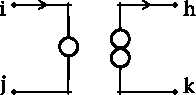
\includegraphics[scale=1]{immagini/nullor.pdf}}
 \caption{Nullatore, noratore e nullore}
 \label{fig:nullorcmp}
\end{figure}

Ancora prima di parlare degli altri componenti, è utile introdurre due elementi che aiuteranno nella comprensione di quanto segue, ovvero il nullatore e il noratore, oltre alla loro diretta estensione, il nullore, osservabili in figura \ref{fig:nullorcmp}.\\
Il nullatore, figura \ref{fig:nullator}, è descritto da \cite{Wikipedia} come:
\begin{quote}
 Un bipolo teorico lineare tempo invariante definito da una corrente e una tensione nulle ai propri capi. Presenta contemporaneamente le proprietà di un corto circuito (tensione nulla) e di un circuito aperto (corrente nulla). Non si comporta né come generatore di corrente né come generatore di tensione, sebbene sia entrambi allo stesso tempo. L'inserimento di un nullatore in un circuito schematico impone vincoli matematici sul comportamento di quest'ultimo, forzando il circuito stesso ad adottare qualsiasi comportamento possibile per far fronte alle richieste. Per esempio l'ingresso di un amplificatore operazionale si comporta come un nullatore, poiché non presenta né assorbimento di corrente né tensione fra i due terminali.
\end{quote}
Il noratore, figura \ref{fig:norator}, è descritto da \cite{Wikipedia} come:
\begin{quote}
 Un bipolo teorico lineare tempo invariante definito da una corrente e una tensione arbitrari ai propri capi. Un noratore rappresenta un generatore controllato di tensione o di corrente con guadagno infinito. L'inserimento di un noratore in un circuito schematico fornisce corrente e tensione a qualsiasi componente esterno le richieda. Per esempio l'uscita di un amplificatore operazionale si comporta come un noratore, producendo tensioni e correnti che soddisfano le richieste del circuito a valle, a discapito di un ingresso nullo.
\end{quote}
Entrambi i componenti se presi singolarmente rappresentano elementi privi di significato. Sono solitamente utilizzati in stretta associazione l'uno con l'altro per definire elementi composti più complessi. Combinandoli in parallelo si ottiene il bipolo corto circuito, mentre la combinazione in serie da luogo ad un bipolo circuito aperto. L'uso più comune è però quello della combinazione come quadripolo (rete 2-porte) ideale, ovvero il nullore riportato in figura \ref{fig:nullor}, dove vengono posti un nullatore in ingresso e un noratore in uscita. Il nullore rappresenta un amplificatore ideale con guadagni di corrente, tensione, transconduttanza e transimpedenza infiniti, i cui parametri di trasmissione possono essere riassunti nella forma matriciale che segue:
$$
\left(
 \begin{array}{c}
  V_{in} \\ I_{in}
 \end{array}
\right)
=
\left(
 \begin{array}{cc}
  0 & 0 \\ 0 & 0
 \end{array}
\right)
\left(
 \begin{array}{c}
  V_{out} \\ I_{out}
 \end{array}
\right)
$$
Per la sua struttura intrinseca e a causa delle imposizioni dettate da nullatore e noratore, il nullore non assorbe corrente e non sussite alcuna differenza di potenziale ai suoi capi. Fra i due terminali sono imposte alcune condizioni sul comportamento, forzando lo schema a far sì che le relazioni costitutive presenti fra loro siano rispettate. Questo lo si può riassumere nella sintesi sotto forma di grafo in corrente e in tensione come segue:
\begin{itemize}
 \item I due nodi ai capi del nullatore collassano nel grafo in tensione.
 \item I due nodi ai capi del noratore collassano nel grafo in corrente.
\end{itemize}
Poiché quanto sopra non è evidentemente possibile (i due nodi sono e devono restare distinti, anche all'interno della coppia di grafi), si forza la presenza dei rami relativi al componente in ognuno degli alberi comuni fra i grafi in corrente e in tensione.\graffito{Il collasso fra vertici può essere simulato forzando un arco fittizio che li unisca negli alberi di copertura, poiché questo preclude la presenza negli alberi stessi di ogni altro arco presente fra i due vertici} In altri termini l'algoritmo di ricerca degli alberi comuni, trattato in seguito, dovrà forzare preventivamente in essi la presenza dei rami nullatore per il grafo in tensione e dei rami noratore per il grafo in corrente, di fatto definendo una radice comune per ogni albero che verrà a formarsi. 

\begin{figure}[b]
 \centering
 \subfloat[A.O.]{\label{fig:ao}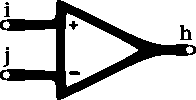
\includegraphics{immagini/opampl.pdf}}\\
 \subfloat[G.I.]{\label{fig:aogi}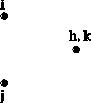
\includegraphics{immagini/nullorgi.pdf}}\hspace{50pt}
 \subfloat[G.V.]{\label{fig:aogv}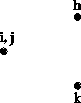
\includegraphics{immagini/nullorgv.pdf}}
 \caption{Rappresentazione di un amplificatore operazionale}
 \label{fig:aocmp}
\end{figure}

In figura \ref{fig:aocmp} è illustrata graficamente la gestione di un amplificatore operazionale ideale (\ref{fig:ao}) nella sintesi sotto forma di grafo in corrente (\ref{fig:aogi}) e grafo in tensione (\ref{fig:aogv}). Se ne ricava un componente costituito, come introdotto in precedenza, da una coppia nullatore-noratore (nullore) dislocati rispettivamente fra i nodi $i$, $j$, $h$ e massa (che sostituisce di fatto il vertice $k$). Concludendo con la parentesi su questa tipologia di componenti particolari basti sapere che, come verrà illustrato in seguito, il nullore è strettamente coinvolto nella rappresentazione non solo dell'amplificatore operazionale ma anche di gran parte dei generatori controllati.

\paragraph{Generatori controllati e non}

\begin{figure}[t]
 \centering
 \subfloat[VCCS]{\label{fig:vccs}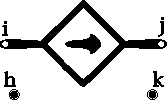
\includegraphics{immagini/vccs.pdf}}\\
 \subfloat[G.I.]{\label{fig:vccsgi}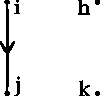
\includegraphics{immagini/vccsgi.pdf}}\hspace{50pt}
 \subfloat[G.V.]{\label{fig:vccsgv}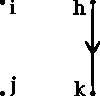
\includegraphics{immagini/vccsgv.pdf}}
 \caption{Generatore di corrente controllato in tensione}
 \label{fig:vccscmp}
\end{figure}

Leggermente più complessa la sintesi dei generatori controllati.\\
La forma più semplice è data dal generatore di corrente controllato in tensione\graffito{Generatore di corrente controllato in tension o VCCS (Voltage Controlled Current Source)}, in figura \ref{fig:vccs}, a causa della sua equazione costitutiva. Come si può osservare, il contributo apportato consiste nell'aggiunta di un arco fra i nodi d'ingresso (\ref{fig:vccsgv}) nel grafo in tensione e un arco fra i terminali d'uscita nel grafo in corrente (\ref{fig:vccsgi}). Per inciso questo è l'unico generatore controllato sintetizzato direttamente, poiché negli altri casi si è dovuti ricorrere a modelli alternativi per riuscire a sposare le richieste degli algoritmi a valle.

\begin{figure}[b]
 \centering
 \subfloat[CCVS]{\label{fig:ccvs}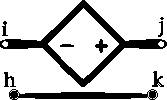
\includegraphics{immagini/ccvs.pdf}}\\
 \subfloat[Circuito equivalente]{\label{fig:ccvseq}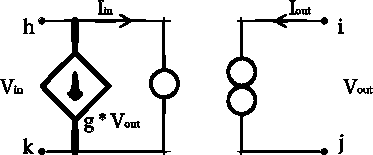
\includegraphics{immagini/ccvseq.pdf}}
 \caption{Generatore di tensione controllato in corrente}
 \label{fig:ccvscmp}
\end{figure}

In figura \ref{fig:ccvscmp} è riportato un generatore di tensione controllato in corrente\graffito{Generatore di tensione controllato in corrente o CCVS (Current Controlled Voltage Source)} (\ref{fig:ccvs}) ed il suo modello equivalente (\ref{fig:ccvseq}), realizzato con i componenti visti precedentemente. Non viene riportata, poiché intuibile, la rappresentazione in forma di grafo in corrente e grafo in tensione, sebbene essa sia direttamente ricavabile da quanto detto a proposito del generatore di corrente controllato in tensione e del nullore. Più precisamente, il generatore di tensione controllato in corrente vedrà:
\begin{itemize}
 \item un arco nel grafo in tensione fra i nodi $h$ e $k$ e uno fra $i$ e $j$ nel grafo in corrente, dovuti al nullore (che, ricordiamo, dovranno essere forzati in ogni albero comune).
 \item un arco nel grafo in tensione fra i nodi $i$ e $j$ e uno fra $h$ e $k$ nel grafo in corrente, dovuti al generatore di corrente controllato in tensione.
\end{itemize}
La relazione costitutiva del modello equivalente risulta essere:
$$ V_{out} = \frac{V_{in}}{g};\quad I_ {in} = 0; $$

\begin{figure}[t]
 \centering
 \subfloat[VCVS]{\label{fig:vcvs}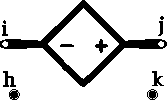
\includegraphics{immagini/vcvs.pdf}}\\
 \subfloat[Circuito equivalente]{\label{fig:vcvseq}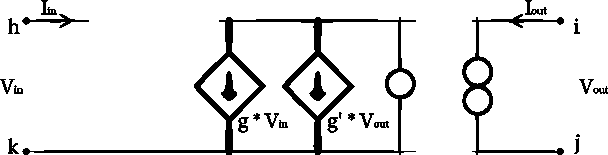
\includegraphics{immagini/vcvseq.pdf}}
 \caption{Generatore di tensione controllato in tensione}
 \label{fig:vcvscmp}
\end{figure}

Discretamente più complesso il modello equivalente del generatore di tensione controllato in tensione\graffito{Generatore di tensione controllato in tensione o VCVS (Voltage Controlled Voltage Source)}, riportato in figura \ref{fig:vcvscmp}. Per la rappresentazione scelta, infatti, si ha la necessità di coinvolgere un nodo ulteriore (oltre ai quattro terminali di ingresso/uscita) dove saranno agganciati i due generatori controllati ed il nullatore. Posto che sia $l$ l'etichetta di tale nodo, in questo caso avremo, a seconda dei componenti coinvolti:
\begin{itemize}
 \item un arco nel grafo in tensione fra i nodi $h$ e $k$ e uno fra $i$ e $j$ nel grafo in corrente, dovuti al nullore (che, ricordiamo, dovranno essere forzati in ogni albero comune).
 \item un arco nel grafo in tensione fra i nodi $i$ e $j$ e uno fra $l$ e $k$ nel grafo in corrente, dovuti ad uno dei due generatori di corrente controllati in tensione.
 \item un arco nel grafo in tensione fra i nodi $h$ e $k$ e uno fra $l$ e $k$ nel grafo in corrente, dovuti al secondo dei due generatori controllati.
\end{itemize}
La relazione costitutiva del modello equivalente risulta essere:
$$ V_{out} = -\frac{g}{g'}\ast V_{in};\quad I_ {in} = 0; $$

\begin{figure}[b]
 \centering
 \subfloat[CCCS]{\label{fig:cccs}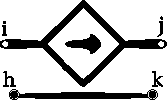
\includegraphics{immagini/cccs.pdf}}\\
 \subfloat[Circuito equivalente]{\label{fig:cccseq}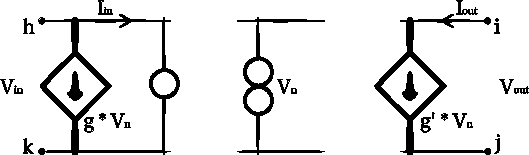
\includegraphics{immagini/cccseq.pdf}}
 \caption{Generatore di corrente controllato in corrente}
 \label{fig:cccscmp}
\end{figure}

Altrettanto complesso il modello equivalente del generatore di corrente controllato in corrente\graffito{Generatore di corrente controllato in corrente o CCCS (Current Controlled Current Source)}, riportato in figura \ref{fig:cccscmp}. Anche in questo caso, come già per il componente visto in precedenza, si ha la necessità di sfruttare un nodo fittizio al quale verrà agganciato il noratore. Posto anche stavolta che sia $l$ tale nodo, avremo:
\begin{itemize}
 \item un arco nel grafo in tensione fra i nodi $h$ e $k$ e uno fra $l$ e $k$ nel grafo in corrente, dovuti al nullore (che, ricordiamo, dovranno essere forzati in ogni albero comune).
 \item un arco nel grafo in tensione fra i nodi $l$ e $k$ e uno fra $h$ e $k$ nel grafo in corrente, dovuti ad uno dei due generatori di corrente controllati in tensione.
 \item un arco nel grafo in tensione fra i nodi $l$ e $k$ e uno fra $i$ e $j$ nel grafo in corrente, dovuti al secondo dei due generatori controllati.
\end{itemize}
La relazione costitutiva del modello equivalente risulta essere:
$$ I_{out} = -\frac{g}{g'}\ast I_{in};\quad V_ {in} = 0; $$

Può forse sembrare fuorviante complicare la rappresentazione di elementi di per sé rappresentabili in modi più sintetici, sotto forma di grafo in corrente e in tensione. In letteratura, infatti, non mancano modelli alternativi che non coinvolgano così tanti componenti. Ciò nonostante va detto che quanto sopra descritto, rappresentato nei diversi modelli equivalenti, si adatta perfettamente alle necessità dell'algoritmo per la ricerca degli alberi comuni a valle del processo di sintesi. Il numero di archi inseriti nei due diversi grafi relativi al circuito, cioè grafo in tensione e grafo in corrente, è infatti lo stesso e tali archi sono sempre dislocati a gruppi fra stessi insiemi di terminali; se ne deduce che i due grafi avranno infine uno stesso numero di nodi e di archi. Questa condizione è, come spiegato in seguito, alla base del funzionamento dell'algoritmo di ricerca degli alberi comuni fra due grafi. Anche la richiesta di terminali ulteriori, fittizi è limitata e non conduce in alcun caso a discostamenti dalle condizioni citate.

\paragraph{}

\begin{figure}[b]
 \centering
 \subfloat[Generatore di tensione]{\label{fig:vgen}
\includegraphics{immagini/voltage.pdf}}\hspace{50pt}
 \subfloat[Generatore di corrente]{\label{fig:igen}
\includegraphics{immagini/current.pdf}}
 \caption{Generatori}
 \label{fig:gens}
\end{figure}

Dall'analisi appena effettuata sembrano mancare due dei componenti più importanti, ovvero i generatori di tensione (figura \ref{fig:vgen}) e i generatori di corrente (figura \ref{fig:igen}). Per quanto riguarda la loro inclusione all'interno del processo di sintesi, è stato scelto un approccio particolare. L'idea alla base è quella di inserire all'interno di ogni singolo circuito un generatore fittizio i cui parametri, opportunamente fissati, non influenzino in alcun modo eventuali generatori da esso controllati. In altri termini il generatore fittizio (per essere precisi, un generatore di tensione)\graffito{Un procedimento simile può essere applicato adottando come riferimento anche un generatore di corrente} è tale per cui, ad esempio, le correnti e le tensioni dei generatori controllati da esso possono essere definite semplicemente attraverso un'oculata politica di assegnazione dei parametri di controllo. Questo fa sì che non vi sia più bisogno di trovare un modello diretto o indiretto per la rappresentazione dei generatori di corrente e di tensione, bensì basterà renderli intelligentemente controllati dal generatore fittizio.\\
Consideriamo per esempio di voler inserire nel circuito un generatore di tensione $V$, questo lo si renderà direttamente controllato dal generatore di tensione fittizio $V_f$. Otteniamo un generatore di tensione controllato in tensione, che sappiamo come trattare, con la necessità di impostare opportunamente i parametri. Supponendo una tensione per $V_f$ pari a $1$ (dalla figura \ref{fig:vcvs}, $V_{in} = 1$), basterà porre $g'$ pari a $-1$ e $g$ pari al valore che si intende assegnare a $V$, ottenendo così quanto desiderato da:
$$ V = -\frac{g}{g'}\ast V_{f};$$
Intuitivamente, questo trucco ha un prezzo da pagare. Il rovescio della medaglia è la necessità di ulteriori terminali fra cui porre il generatore fittizio (ovvero almeno un terminale) col conseguente aumento di complessità per la gestione di generatori di corrente e di tensione non controllati come generatori controllati. Questo si traduce in una lieve crescita nella dimensione dei due grafi in corrente e in tensione associati al circuito, e quindi in un maggiore sforzo computazionale per la risoluzione.

\paragraph{}

\begin{figure}
 \centering
 \subfloat[Modello]{\label{fig:transformer}
\includegraphics{immagini/transformer.pdf}}\hspace{50pt}
 \subfloat[Circuito equivalente]{\label{fig:transeq}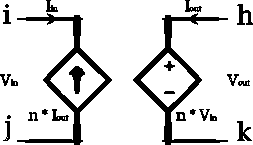
\includegraphics{immagini/transformereq.pdf}}
 \caption{Rappresentazione di un trasformatore ideale}
 \label{fig:trans}
\end{figure}

Proseguendo nella carrellata sui componenti disponibili per il disegno schematico e in particolare su quelli creati a partire dai generatori controllati, in figura \ref{fig:trans} sono riportati componente e circuito equivalente relativi ad un trasformatore ideale. Nel caso specifico ci si ricollega al modello generale, valido a prescindere, del trasformatore ideale, composto appunto da due generatori controllati incrociati (un generatore di corrente controllato in corrente ed un generatore di tensione controllato in tensione), ovvero tali da far sì che i terminali di controllo del primo rappresentino i terminali di uscita del secondo e viceversa. Anche in questo caso, a parte alcuni accorgimenti specifici a livello di programmazione, utili a rendere effettivamente sensibile il componente alla corrente di controllo (si ha la necessità di un nodo fittizio di corredo), si è aggiunto un nuovo elemento sfruttando esclusivamente ciò di cui già disponevamo, alleggerendo il tutto tanto a livello teorico quanto pratico.

\begin{figure}
 \centering
 \subfloat[Modello]{\label{fig:mutualinductance}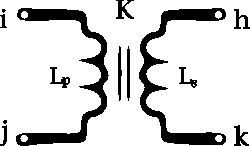
\includegraphics{immagini/mutualinductance.pdf}}\\\vspace{25pt}
 \subfloat[Circuito equivalente]{\label{fig:mutindeq}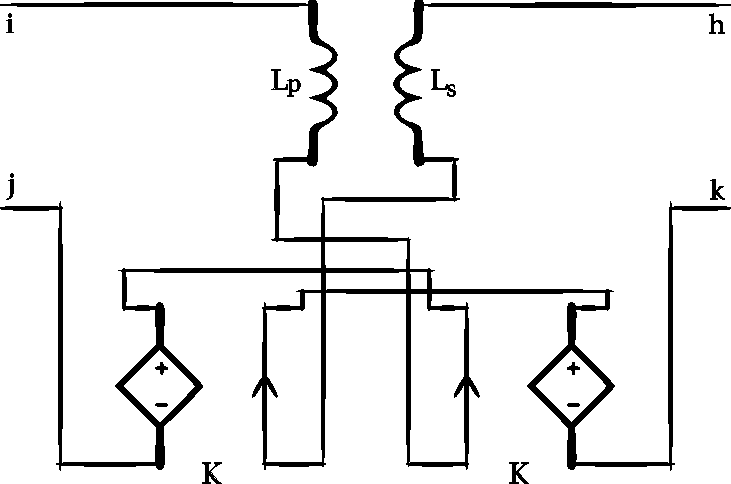
\includegraphics[scale=0.65]{immagini/mutualinductanceeq.pdf}}
 \caption{Rappresentazione di una mutua induttanza}
 \label{fig:mutind}
\end{figure}

Un procedimento simile, sviluppato attraverso l'aggiunta di nodi fittizi e altri piccoli accorgimenti a livello software, riguarda la mutua induttanza (riportata in figura \ref{fig:mutind} e in forma simbolica in \ref{fig:mutualinductance}). In questo caso si fa uso di generatori di tensione controllati in corrente accoppiati con induttori e si ha la necessità di ben quattro nodi fittizi. Ancora più importante, nell'esempio, il fatto che per un corretto funzionamento bisogna agire aggirando la corretta modalità di apporto dei dati da parte dei generatori controllati, forzando per essi un grado pari a $1$ per la variabile libera $s$ (sarebbe normalmente $0$). Questo è necessario poiché essi vanno a sostituire quello che sarebbe un altro induttore nel modello passivo alternativo e concorrono, nello schema equivalente in figura \ref{fig:mutindeq}, a mettere in relazione fra loro i due induttori componenti della mutua induttanza.

\paragraph{Conclusione}
Attraverso quanto illustrato nei paragrafi precedenti si è visto come, attraverso quelli che sono pochi oggetti elementari quali resistenze, ammettenze o nullori, si riescano a comporre elementi ben più complessi come ad esempio i generatori controllati. A partire da questi, inoltre, si sono realizzati ulteriori componenti come composizione di elementi aggregati, il che rende fede all'idea che attraverso questa tecnica tutto ciò che è modellabile con gli oggetti base è di fatto realizzabile in termini di grafi equivalenti. Pertanto, sebbene non risultino direttamente realizzabili elementi quali ad esempio i transistori, ne sono perfettamente modellabili i loro circuiti equivalenti come quello per piccoli segnali. Questo dovrebbe far intuire la flessibilità e la capacità espressiva di uno strumento in grado di dar luogo all'analisi simbolica, basti pensare infatti che attraverso di esso si possono potenzialmente analizzare tutti quei circuiti che sono esprimibili come modelli equivalenti contenenti gli elementi base accettati dal sistema.

\chapter{Metodo dei due grafi}

\section{Teoria}

Il metodo dei due grafi è ad oggi forse la tecnica più performante per la risoluzione del problema dell'analisi simbolica. Questo metodo si appoggia alla rappresentazione di un circuito elettrico tramite l'uso di due grafi detti \textbf{Grafo in Corrente (gI)} e \textbf{Grafo in Tensione (gV)}. Come visto in precedenza, i due grafi ottenuti dalla sintesi dei componenti presenti nel circuito hanno stessa cardinalità per quanto riguarda l'insieme dei nodi e quello degli archi. Se si considera inoltre il processo di costruzione adottato, si possono trarre interessanti conclusioni:
\begin{itemize}
 \item I grafi \textit{gI} e \textit{gV} hanno, appunto, uno stesso numero di nodi e uno stesso numero di archi
 \item Un albero per \textit{gI} ha lo stesso numero di archi di un albero per \textit{gV} e viceversa, pari al numero di nodi diminuito di uno
 \item Per costruzione, laddove l'$i_{esimo}$ arco di \textit{gI} si riferisca ad un componente $C$, allora anche l'$i_{esimo}$ arco di \textit{gV} si riferirà a quello stesso componente (questo perché i componenti introducono uno stesso numero di archi in ogni grafo e si suppone che gli archi vengano etichettati in base all'ordine di inserimento)
\end{itemize}
Nota: dall'ultimo punto si deduce che le informazioni non necessitano di essere duplicate, bensì condivise fra i singoli archi che si corrispondono nei due grafi, il che contribuisce ad abbattere ulteriormente lo spazio richiesto per la memorizzazione.

Molto importante, pertanto degno di essere ribadito ancora una volta, è il fatto che gli archi debbano essere etichettati, immagazzinati o comunque recuperabili nello stesso ordine di immissione. Su questo punto, infatti, si basa l'intero algoritmo che sarà illustrato di seguito e questo stesso aspetto rappresenta spesso un approccio scarsamente considerato nell'uso di grafi. Osservando la questione dal punto di vista opposto, si può formulare un enunciato come segue:

\paragraph{}
\emph{
Siano $gI^L$ e $gV^L$ due liste di archi aventi stessa cardinalità e sulle quali sia indotto un ordinamento (ad esempio basato sulla posizione occupata nella lista), supposto che gli archi siano definiti su uno spazio di vertici avente cardinalità $N$ in entrambi i casi, allora si ha che:
\begin{itemize}
 \item Le due liste concorrono a definire due grafi distinti, \textit{gI} e \textit{gV}, composti rispettivamente dai due elenchi di archi, aventi stessa cardinalità tanto in numero di vertici quanto in numero di archi.
 \item Un albero comune è dato da un insieme di indici $I^T$ di cardinalità $N-1$ tale che, sfruttando gli ordinamenti indotti sulle due liste, gli archi individuati da tali indici in ognuna di esse descrivono un albero sul grafo corrispondente.
 \item Un insieme di indici $I^E$ di cardinalità $N-1$ tale che gli archi individuati nelle due liste formano solamente in uno dei due casi un albero per il grafo corrispondente, non si può definire tale da descrivere un albero comune
\end{itemize}
}

\paragraph{}

\begin{figure}[b]
 \centering
 \subfloat[Grafo in corrente]{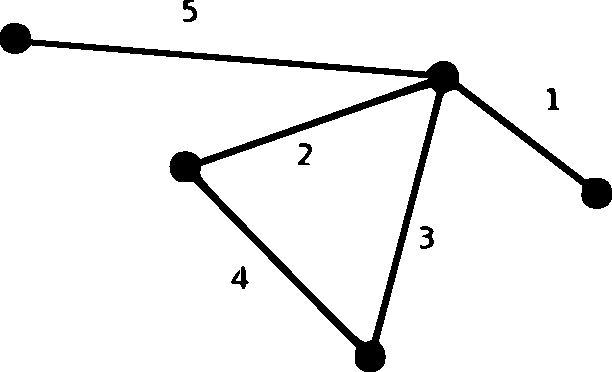
\includegraphics[scale=0.5]{immagini/gi.pdf}}
 \hspace{25pt}
 \subfloat[Grafo in tensione]{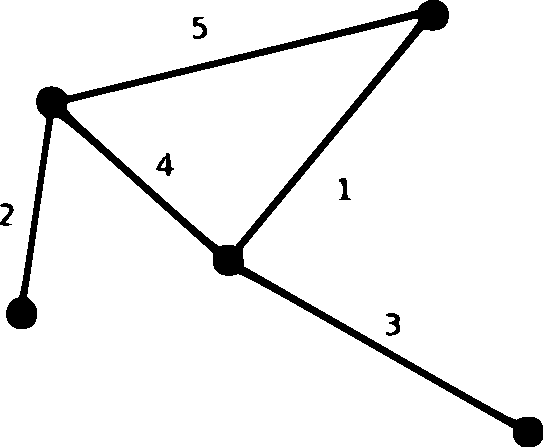
\includegraphics[scale=0.5]{immagini/gv.pdf}}
 \caption{Coppia di grafi con alberi in comune}
 \label{fig:gigv}
\end{figure}

Data la semplicità del concetto ma la sua difficoltà di esposizione, si procede con un esempio. Osserviamo la figura \ref{fig:gigv}, dove sono descritti due grafi che possono essere derivati dalla sintesi di un circuito elettrico. Gli archi sono numerati, per costruzione, in base all'ordine di immissione e pertanto l'arco $1$ nel primo e nel secondo grafo sarà legato allo stesso pacchetto di informazioni esterne all'algoritmo di ricerca degli alberi comuni. Cambiando punto di vista, se l'informazione viene scelta, ciò implica che i due archi etichettati con $1$ vengono scelti.\\
Con una semplice occhiata si nota che i due grafi hanno almeno un albero in comune, dato dagli archi etichettati con $1-2-3-5$. Dalle ipotesi sopra, restituendo questo insieme di indici al richiedente, sarà sufficiente accedere ai blocchi di dati legati al singolo indice per recuperare le informazioni necessarie, senza dovere ulteriormente interagire con la coppia di grafi che (a parte l'etichetta associata al singolo arco) niente sanno delle informazioni presenti.

\paragraph{}
Riassumendo, quindi, l'idea è quella di costruire in maniera idonea i due grafi, così che si possano dare in pasto ad un algoritmo di ricerca degli alberi comuni che non debba preoccuparsi dei dati legati ai singoli archi, poiché a priori non ci sono riserve sull'inclusione o esclusione di una coppia di archi legati fra loro. Su tali presupposti si può quindi operare ottenendo una lista di alberi in comune a partire dalla quale, in seguito, sarà estrapolata la soluzione cercata con tecniche apposite che esulano dall'obiettivo dell'algoritmo di ricerca.\\
Di seguito verranno illustrati due algoritmi, uno il miglioramento dell'altro, che mirano appunto a individuare alberi in comune fra grafi descritti come lista di archi, pertanto è compito dell'utente costruire in maniera attenta tale lista.



\section{Il metodo di Grimbleby}

Questo primo metodo è descritto in \cite{Grimbleby} e, sebbene sia stato usato largamente e per molti anni (anche e soprattutto in Sapec), soffre di alcune carenze dal punto di vista dell'ottimizzazione. Come vedremo in seguito, infatti, con pochi semplici accorgimenti si può evitare di percorrere alcune strade che si rivelano a priori sterili, alla ricerca di alberi in comune.\\
Ciò nonostante, per quello che ha rappresentato nel campo dell'analisi simbolica, l'algoritmo di Grimbleby deve essere introdotto, poiché ha il merito di definire una base di partenza per lo sviluppo di molte altre metodologie più performanti.

L'algoritmo di Grimbleby\graffito{Il metodo di Grimbleby prende il nome dal suo autore, James B. Grimbleby, e si basa sui risultati ottenuti da Nicos Christofides nel campo della teoria dei grafi} è stato concepito in seno al problema dell'analisi simbolica e quindi costruito sulle ipotesi sopra elencate, per quanto riguarda i due elenchi di archi. Parte cioè dal presupposto che siano definiti due grafi (di tensione e di corrente) aventi stesso numero di nodi e stesso numero di archi e tali che su questi ultimi sia indotto un ordinamento di qualche genere. Il metodo è basato sull'algoritmo di ricerca di un albero di copertura per un grafo come descritto in \cite{GraphTheory} che, come indicato anche dall'autore stesso, è probabilmente inferiore in termini di prestazioni rispetto ad altri algoritmi. Di seguito è riportato l'algoritmo proposto originale, corredato di alcune condizioni a monte e alcune note sulle strutture dati.

\paragraph{}
\emph{
Supponiamo di avere due grafi, $G1$ e $G2$, composti da $N$ nodi e $M$ archi. Inoltre, supponiamo di poterci appoggiare a due grafi inizialmente costituiti dai soli vertici e privi di archi (grafi di questo tipo vengono detti anche foreste), chiamati $H1$ e $H2$. Infine, si utilizzerà uno stack $S$ di capacità pari a $N-1$ ed un contatore $K$ (quest'ultimo è indicato come \textit{puntatore ad arco}, nel senso che mantiene l'indice di riferimento dell'arco in esame). L'algoritmo si sviluppa in pochi semplici passi ed è facilmente implementabile come macchina a stati (tecnica seguita in SapecNG):
\begin{enumerate}
 \item \textbf{Inizializzazione:} $H1$ e $H2$ non contengono inizialmente archi e sono considerati come foreste di $N$ alberi (in altre parole, ogni arco non connesso è considerato un albero e così lo sarà anche nel seguito), lo stack è svuotato e $K$ è posto a $0$.
 \item \textbf{Controllo per albero comune:} se nello stack sono presenti $N-1$ archi, allora è stato individuato un albero comune; gestirlo (o memorizzarlo) e passare al punto 7.
 \item \textbf{Selezione di un nuovo arco:} Incrementare $K$ ($K = K+1$); se non vi è un numero sufficiente di archi per completare un albero (ovvero, $size(stack) + M - K < N - 2$) passare al punto 6.
 \item \textbf{Controllo generazione ciclo:} se l'arco $K$ di $G1$ ($G2$) genera un ciclo in $H1$ ($H2$), allora passare al punto 3.
 \item \textbf{Inclusione arco:} porre $K$ in cima allo stack, quindi includere l'arco $K$ di $G1$ ($G2$) in $H1$ ($H2$). Sia in $H1$ che in $H2$ questo comporterà la fusione di due alberi in uno solo.
 \item \textbf{Controllo completamento:} se lo stack è vuoto, l'algoritmo è concluso e tutti gli alberi di copertura comuni sono stati individuati e gestiti o memorizzati.
 \item \textbf{Backtrack:} rimuovere un arco dalla cima dello stack $S$, quindi porre $K$ pari ad esso; rimuovere l'arco $K$ di $G1$ ($G2)$ da $H1$ ($H2$), il che concorrerà a suddividere in $H1$ ($H2$) un singolo albero in due alberi distinti. Passare al punto 3.
\end{enumerate}
}

\paragraph{}
I grafi $G1$ e $G2$ non richiedono una particolare struttura dati e viene consigliato un immagazzinamento sotto forma di due liste di $M$ coppie di nodi. Per quanto riguarda $H1$ e $H2$, invece, è consigliata l'individuazione di una struttura dati che faciliti le seguenti operazioni:
\begin{itemize}
 \item Controllo nel caso in cui un particolare arco (quando aggiunto in $H1$ o $H2$) generi un ciclo; ciò è equivalente a controllare dove i due archi componenti appartengono già ad uno stesso albero.
 \item Inclusione di un arco con conseguente connessione di due alberi, quindi fusione di questi ultimi in un singolo albero.
 \item Rimozione di un arco, quindi scissione di un albero in due alberi distinti.
\end{itemize}
In \cite{Grimbleby} è proposta la soluzione descritta di seguito. Si crei una lista di cardinalità $N$ per ognuno dei grafi, i cui componenti sono coppie di puntatori:
$$(R_j, P_j), \forall j=1\dots N$$
In ogni albero del grafo un vertice è scelto in modo arbitrario per essere il nodo radice: $R_j$ è la radice dell'albero a cui il nodo $j$ appartiene, mentre $P_j$ è il diretto antenato del nodo $j$ ed è tale che la coppia $(j, P_j)$ rappresenti un arco valido (i nodi radice sono eccezioni e non hanno antenati, in altri termini si può porre come loro antenato sé stessi). Tale lista di $N$ coppie radice e antenato definisce completamente il grafo e si presta in modo particolare ad essere maneggiata facilmente sulla base delle richieste fatte in precedenza.

Inizialmente poiché $H1$ e $H2$ non contengono archi e ogni vertice è considerato un albero a sé stante, ogni nodo è la propria radice e non ha predecessori, ovvero:
$$ \forall j=1\dots N : R_j = j, P_j = 0 $$
Quindi, i tre punti di cui sopra si risolvono banalmente come segue:
\begin{itemize}
 \item La generazione di un ciclo durante l'aggiunta di un arco $(i, j)$ può essere individuata semplicemente controllando se $R_i$ e $R_j$ hanno uno stesso valore, poiché se così fosse allora si può dedurre che $i$ e $j$ appartengano ad uno stesso albero. Segue che l'aggiunta dell'arco $(i, j)$ genererà inevitabilmente un ciclo.
 \item L'inclusione di un arco $(i, j)$ e quindi la fusione di due alberi in uno solo richiede:
           \begin{description}
            \item[Modifica radici sui vertici] Tutti i nodi con radice $R_j$ la vedano cambiata in $R_i$.
            \item[Modifica radice sull'albero] Gli antenati sul cammino fra $j$ e $R_j$ vengano ribaltati, questo renderà $j$ radice dell'albero.
            \item[Modifica antenato] $P_j$ venga cambiato in $i$.
           \end{description}
 \item La rimozione di un arco $(i, j)$ e quindi la scissione di un albero in due alberi distinti richiede:
           \begin{description}
            \item[Normalizzazione indici] Siano scambiati $i$ e $j$ laddove $P_j \neq i$, così che si abbia $P_j = i$.
            \item[Scissione] Siano posti $P_j = 0$ e $R_j = j$, ovvero $j$ diventi la radice dell'albero disconnesso.
            \item[Correzione radici] Considerando ogni nodo $l$ in $\{ 1\dots N\}$ ad eccezione di $j$, se $R_l \neq j$ e $R_{P_l} = j$ allora si ponga $R_l = j$. Questo passo deve essere ripetuto sui vertici fintanto che avvengono modifiche sulle radici.
           \end{description}
\end{itemize}

\paragraph{}
Nonostante gli sforzi per proporre strutture dati idonee, l'algoritmo di Grimbleby soffre come già anticipato di una grave mancanza: un controllo aprioristico che gli permetta di potare i rami del proprio cammino evitando di percorrere strade sterili. Ciò lo rende notevolmente meno performante di quello incluso in QSapecNG che, per onor di cronaca, è concepito a partire da quello sopra proposto che appunto funge da base e punto di partenza per questa branca di algoritmi su grafi. 

Una implementazione in C per SapecNG dell'algoritmo di Grimbleby esiste ed è pensata come macchina a stati, poiché per la sua struttura ed esposizione si presta in maniera particolare. Le richieste in termini di occupazione di memoria per le proprie strutture dati non sono esose, sebbene mantenere due grafi paralleli ($H1$ e $H2$) per facilitare la costruzione degli alberi possa incidere notevolmente sul conto finale, soprattutto nel caso in cui si affrontino grafi $G1$ e $G2$ di dimensioni molto grandi (come è plausibile aspettarsi, un po' perché dimensioni piccole indicano un circuito associato molto piccolo, che quindi non ha bisogno di un software apposito per essere studiato e un po' perché molti componenti includono più di un arco in ognuno dei due grafi, il che ne facilita l'esplosione).

In \cite{Schach} viene fatta un'analisi di tale algoritmo e viene dimostrato come, ad esempio, se ne possano aumentare le performance fino al 50\% semplicemente utilizzando una struttura dati doppiamente collegata tramite puntatori per la memorizzazione degli alberi, il che rende facilmente un'idea delle lacune del metodo di Grimbleby.


\section{Il metodo di Schach}

Questo secondo metodo si sviluppa a partire dall'algoritmo di Grimbleby e viene descritto nel dettaglio in \cite{MRT}. Del suo predecessore eredita gli spunti più interessanti e l'idea di fondo, aggiungendo alcune tecniche che limitino le richieste di occupazione per le strutture dati e che siano in grado di prevenire la ricerca di alberi su percorsi che si possono individuare come sterili a priori. Alla base vi è il riconoscimento che l'algoritmo di Grimbleby si basa completamente su un metodo inefficiente \cite{GraphTheory} e quindi già di partenza ha un corredo di svantaggi in eredità. Come conseguenza nel caso peggiore si ha la generazione di un numero altissimo di plausibili alberi comuni che, in realtà, si rivelano tali soltanto in parte e pertanto concorrono ad uno spreco notevole di energie per la loro generazione e distruzione. L'algoritmo qui descritto, invece, affonda le sue radici in quanto proposto con \cite{Minty} e formalizzato con \cite{ReadTarjan}, ovvero un metodo efficiente per la ricerca su singolo grafo. Basti pensare che il metodo di Schach migliora le performance dell'algoritmo di Grimbleby di un fattore che oscilla fra 350\% e 26.000\%, a seconda delle situazioni che gli si presentano. Ne consegue che, inevitabilmente, si spalancano le porte alla risoluzione di circuiti molto più complessi di quanto il metodo di Grimbleby non permettesse di affrontare.

\graffito{L'algoritmo proposto da Stephen R. Schach prende il nome dagli autori di un altro algoritmo, che sta alla base dell'idea sviluppata in esso come miglioria al metodo di Grimbleby, ovvero Mint, Read e Tarjan}Dal nome degli autori dell'algoritmo su cui il metodo di Schach si basa, quest'ultimo prende il nome di \textbf{MRT}.

Similmente a quanto proposto da Grimbleby, tutte le possibili combinazioni di $(M-1)$ alberi vengono potenzialmente generate. A differenza del suo predecessore però, questo avviene solo e soltanto potenzialmente: infatti, laddove si incontri un arco $j$ di $G1$ ($G2$) che se aggiunto alla foresta di copertura parziale per $G1$ ($G2$) finisce con l'indurre un ciclo, tale arco è immediatamente rigettato. Con ciò si riduce il numero di possibilità da investigare, poiché rigettare un arco significa potare tutti gli alberi che potevano essere generati a partire dalle foreste di copertura parziali in esame e non vi sarà (non vi potrebbe essere) nessun albero di copertura tale da includere l'arco $j$ e al contempo le foreste di copertura parziali allo stato attuale. In questi casi, l'arco $j$ è etichettato come \textit{induttore di ciclo}.\\
Le differenze principali fra i due algoritmi sono:
\begin{itemize}
 \item L'uso dei \textit{ponti} da parte del metodo di Schach.
 \item La memorizzazione in una lista $L$ degli indici $j$ per gli archi della foresta di copertura parziale corrente (non si ha una costruzione esplicita delle foreste, come avviene per Grimbleby, il che riduce il numero di operazioni e il carico di memoria richiesta necessari).
\end{itemize}

\paragraph{}
Prima di procedere, è utile soffermarsi su cosa siano i ponti e sul mondo che gira loro intorno. Ricordiamo innanzitutto che un grafo $G$ si dice connesso se per ogni coppia di vertici $v$ e $w$ esiste un cammino in grado di unirli. Supposto quindi $G$ connesso, un ponte lo si può definire come un arco $b \in G$ tale che se rimosso da $G$ quest'ultimo non risulta più essere connesso. In altri termini, se $b$ viene rimosso allora $G$ risulterà suddiviso in due componenti connesse completamente indipendenti fra loro, $G_1$ e $G_2$.

Il metodo di Schach sfrutta in modo intelligente i ponti per i suoi scopi in due modi distinti. Prima di tutto si assicura che ogni ponte venga incluso in ogni albero di copertura comune, contenente la foresta di copertura parziale attuale (non potrebbe essere altrimenti e così facendo si tagliano fuori un buon numero di potenziali alberi in realtà nulli). Inoltre se il $j_{esimo}$ arco di $G1$ è un ponte per $G1$ e al contempo il $j_{esimo}$ arco di $G2$ è marcato come induttore di ciclo (ovvero connette due vertici nello stesso albero della foresta di copertura parziale), allora la fase di gestione e regressione comincia immediatamente poiché è ovvio che risulta impossibile soddisfare il requisito per cui tale arco sia incluso ed escluso allo stesso tempo da un potenziale albero di copertura comune.

\lstset{basicstyle=\small, language=pseudocode, breaklines, breakatwhitespace, morekeywords={MRT, REC_MRT, _a, _b}}
\begin{lstlisting}[float, frame=shadowbox, framexleftmargin=3mm, caption=Algoritmo MRT, captionpos=t, label=lst:MRT]
procedura REC_MRT;
inizio
  se L contiene (N-1) archi, allora L contiene un albero di copertura comune per i grafi G1 e G2;
  altrimenti
    inizio
      se esiste un arco j che non sia induttore di ciclo
      allora
        inizio
          aggiungere j a L;
          marcare come cancellati da G1 e G2 tutti gli archi induttori di ciclo; (_a)
          REC_MRT; (invocazione ricorsiva)
          riposizionare in G1 e G2 tutti gli archi precedentemente eliminati al passo (_a);
          rimuovere j da L;
          marcare come cancellato l'arco j in G1 e G2;
          marcare tutti gli archi che si rivelano ponti rispettivamente per G1 e G2; (_b)
          se nessuno degli archi marcati al passo (_b) come ponte di un grafo risulta induttore di ciclo nei confronti dell'altro grafo
          allora
            inizio
              aggiungere tutti gli indici degli archi marcati al passo (_b) in L;
              REC_MRT; (invocazione ricorsiva)
              rimuovere da L gli indici degli archi marcati al passo (_b);
            fine
          riposizionare j rispettivamente in G1 e G2;
        fine
    fine
fine

procedura MRT;
inizio
  inizializzare L inserendo gli indici di tutti gli archi j che si rivelano essere ponti in G1 e/o G2;
  se entrambe le foreste di copertura parziale sono libere da cicli
  allora
    inizio
      cancella tutti gli archi induttori di ciclo da G1 e da G2;
      se G1 e G2 sono ancora entrambi connessi
      allora
        invoca REC_MRT;
    fine
fine
\end{lstlisting}

\paragraph{}
Nel listato \ref{lst:MRT} è riportato l'algoritmo in forma di pseudo-codice, sulla base di quanto proposto in \cite{MRT}. Le definizioni riguardanti $G1$ e $G2$ sono le stesse già viste in precedenza, mentre $L$ rappresenta uno stack in cui sono depositati gli indici delle foreste di copertura parziali e quindi degli alberi di copertura comuni per i due grafi i quali, come è necessario ricordare, non sono costruiti e distrutti in parallelo come avviene invece nell'algoritmo di Grimbleby.\\
L'algoritmo si compone di due procedure: la prima di ingresso e inizializzazione mente la seconda, ricorsiva, rappresenta il vero e proprio cuore dell'algoritmo.

In questa sede non verranno discussi in modo approfondito le migliori metodologie per l'individuazione di cicli, la ricerca di ponti o tutte le altre procedure di secondaria importanza coinvolte nell'algoritmo principale. Si noti invece come già dallo pseudo-codice, per quanto complesso possa sembrare ad una prima occhiata, traspaia il modus operandi introdotto in precedenza.

Nella procedura MRT, infatti, è già presente una prima fase di analisi pre-ricerca (assente nel metodo di Grimbleby) che può portare addirittura a fermare l'algoritmo immediatamente, laddove si rilevi il fatto che non possono esistere per alcun motivo alberi di copertura comuni. Ancora, in essa si può osservare fin dalla prima istruzione l'importanza data ai ponti (in questo frangente, ponti a grafo completo) i quali, per forza di cose, vengono forzati ad essere contenuti in ogni albero di copertura comune.

La procedura REC\_MRT attraversa due fasi ben distinte fra loro, le quali si evolvono entrambe in una fase ricorsiva basata su presupposti ridotti. La prima tende a costruire un albero con le risorse a disposizione, come ci si potrebbe aspettare, ovvero cercando un arco $j$ che sia plausibilmente accettabile per l'inserimento sulla base di criteri ben definiti e sufficientemente chiari. La seconda fase opera in maniera molto particolare. Di fatto l'arco utilizzato nella prima fase viene rimosso, ottenendo così un grafo di cardinalità inferiore per quanto riguarda il numero di archi, poiché necessariamente il $j_{esimo}$ arco ha esaurito ogni suo compito per quanto riguarda l'indice in esame e può essere scartato. L'operazione che segue mima poi quanto avviene nella fase di inizializzazione (procedura MRT), gestendo i ponti e invocando REC\_MRT sul grafo ridotto e con lo stack $L$ pre-inizializzato.

Tale comportamento potrebbe far sorgere dubbi leciti sul perché l'arco $j$ venga scartato, precludendone la possibilità di comparire ancora una volta in alberi di copertura comuni. Il motivo non è del tutto banale e discende dalle considerazioni che seguono. Il $j_{esimo}$ arco è scelto fra $N$ poiché gli archi compresi in $\{ 1\dots j-1\}$ si erano rivelati essere induttori di ciclo oppure cancellati oppure ancora già presenti in L (si noti che queste sono le tre variazioni di stato possibili, oltre alla possibilità di non avere uno stato effettivo e le liste di archi vengono visitate in modo sequenziale, per ipotesi, da cui l'affermazione precedente). Una volta utilizzato il $j_{esimo}$ arco, eliminandolo da $L$ si ha che necessariamente gli archi con indice $i \in \{ 1\dots j-1\}$ tornano ad essere non accettabili per la foresta di copertura parziale, pertanto (supponendo di accedere alla seconda fase ricorsiva) tutti gli archi che vengono aggiunti a $L$ e al contempo sono ponti per $G1$ ($G2$) e non sono induttori di ciclo per $G2$ ($G1$) hanno indice maggiore di $j$ per costruzione. Ne consegue che se esiste un albero di copertura comune che preveda almeno l'insieme di archi aggiunto e $j$, allora tale albero è gia stato individuato nella fase ricorsiva precedente, con radice $j$ e avremmo un duplicato. Pertanto l'esclusione di $j$ non solo è utile per non disperdere energie su strade già battute, bensì si rivela necessaria per aggirare la duplicazione degli alberi di copertura comuni nel caso non vi sia un controllo a posteriori sugli insiemi di indici.\\
Una dimostrazione formale esiste ed è, ovviamente, molto più complessa di quanto spiegato a parole ma esula dallo scopo del lavoro di tesi ed è stata pertanto omessa.

\chapter{Rappresentazione simbolica}

Sulla base di quanto introdotto nei capitoli precedenti, vi sono gli elementi per potersi approcciare ad un circuito e tentarne quella che si potrebbe definire la risoluzione, ovvero l'estrapolazione di valori significativi in formato simbolico legati a grandezze specifiche.\graffito{Per l'approccio descritto è necessario che fra le informazioni associate al singolo arco vi sia un parametro che ne descriva la tipologia, ovvero indichi se si tratta di un componente tipo ammettenza, impedenza o nullore} A questo scopo conviene procedere un passo alla volta, descrivendo nei dettagli il comportamento da adottare con circuiti costituiti da soli componenti con rappresentazione ammettenza e transcoduttanze (detti circuiti $RCg_m$), quindi estendendo l'analisi ai componenti con rappresentazione impedenza e infine a tutti quelli che subiscono le imposizioni dovute alla presenza di nullori nei loro modelli equivalenti.

Sarà illustrata inoltre nel prosieguo la tecnica del circuito modificato, la cui utilità consiste nel dare una separazione netta ai componenti dell'espressione finale, così da poterli individuare,  raggruppare ed utilizzare senza difficoltà.

\paragraph{Circuiti $RCg_m$}
Nel caso specifico avremo, da quanto già ampiamente discusso in precedenza, quanto segue:
\begin{itemize}
 \item I componenti bipolari producono, sui due grafi, un ramo fra gli stessi due nodi. Il loro peso, ovvero l'informazione associata a tali rami, è dato dal valore del componente stesso espresso in formato numerico e/o simbolico (laddove presenti).
 \item La transcoduttanza $g_m$ da luogo a un ramo fra i nodi di controllo nel grafo in tensione, mentre nel grafo in corrente introduce un ramo fra i nodi controllati. Da notare che, ai fini del procedimento di assegnamento dell'informazione, in entrambi i grafi il peso del ramo aggiunto è il valore della transcottudanza stessa (nominale e simbolico).
\end{itemize}
Supponiamo di aver ricavato da un circuito $RCg_m$ il grafo in tensione $gV$ ed il grafo in corrente $gI$. Entrambi i grafi avranno $N$ vertici e $M$ archi ed ogni loro albero di copertura conterrà esattamente $N-1$ archi. Supponiamo inoltre che, a partire dai due grafi e applicando uno dei metodi di ricerca degli alberi comuni, si sia ottenuto un insieme di $k$ alberi di copertura comuni:
$$ T = \{ T_1\ldots T_k \}~\mid~ T_i \in \{0\ldots M - 1\}^{N-1}$$
Per cui valga, dalla definizione di albero:
$$ \forall i = 1\ldots k\quad T_i^j \neq T_i^h\quad,\quad\forall j, h \in\{1\ldots N - 1\} ~\mid~ j \neq h $$

Alla luce di tutto ciò avremo che il determinante della matrice delle ammettenze ai nodi può essere calcolato come:
$$
\Delta =
\sum_{i = 1}^k{
  \varepsilon_i\ast\left(\begin{array}{c}
    prodotto~ammettenze~presenti~su~T_i
  \end{array}\right)
}
$$
Dove si abbia come discriminatore del segno:
$$ \varepsilon_i = \pm 1 $$
$$ \varepsilon_i = \left( det\left[ m\{ A_i \} \right] \right)\ast\left( det\left[ m\{ A_v \} \right] \right) $$
Resta da definire chi siano le due matrici $m\{ A_i \}$ e $m\{ A_v \}$. Altro non sono che le matrici d'incidenza ridotte, relative ai due alberi considerati o meglio alla proiezione sui due grafi dell'albero di copertura comune in esame. Poiché la matrice d'incidenza è riducibile ad una matrice quadrata di rango pari a $N-1$ e proprio a causa dell'unimodularità di tale matrice, il determinante sarà dato dai valori $\pm 1$. In realtà potremmo anche avere un determinante pari a $0$ ma tale caso è stato volutamente ignorato poiché, laddove l'evenienza abbia luogo, la matrice delle ammettenze ai nodi non subisce alcun apporto dall'albero comune in esame. Un tale albero può essere semplicemente scartato.

\paragraph{}
Prima di proseguire ulteriormente su questa strada, bisogna aprire una parentesi importante. Prestando attenzione al procedimento di ricerca degli alberi di copertura comuni e quindi a quello di definizione della matrice delle ammettenze ai nodi, si nota come i grafi in corrente e in tensione associati al circuito debbano essere al contempo orientati e non. A motivazione di ciò osserviamo che l'algoritmo di ricerca degli alberi di copertura comuni agisce e parte dal presupposto di operare su un grafo non orientato, infatti la sola idea dell'uso di ponti perde un po' di significato con grafi orientati dove invece avremmo strutture e componenti con definizioni più forti. Allo stesso tempo, è stato appena spiegato come sia utile ricavare le matrici d'incidenza per calcolare quello che si potrebbe definire il segno della matrice delle ammettenze ai nodi.\\
A tal proposito, per onor di cronaca, viene illustrata la semplice soluzione adottata.\\
Facendo un passo indietro, si riscopre la necessità di memorizzare i singoli grafi come liste di archi. Così facendo, per ottimizzare anche l'uso di memoria, si può immagazzinare il singolo arco come fosse orientato, cercando di essere coerenti nel trattare stessi componenti. A questo punto è possibile gestire l'intero grafo come non orientato, considerando che ogni ramo $\left( i, j\right)$ memorizzato definisce implicitamente anche il ramo $\left( j, i\right)$ non memorizzato. Ciò nonostante, per costruzione, il grafo stesso, o meglio i suoi rami portano con loro l'informazione relativa al proprio orientamento, che in questa sede potremmo meglio definire come \textit{orientamento in fase di inserimento}, utilizzabile quando necessario.

\paragraph{Componenti con rappresentazione impedenza}
Volendo allargare la cosa anche a circuiti con componenti non di tipo ammettenza, quali resistenze e induttori, questo è possibile attraverso pochi, semplici passi.

Bisogna però prima fare una premessa introduttiva. Preso un generico albero $T$ su un grafo $G$, si definisce il coalbero di $T$ la foresta $T'$ composta da tutti e soli gli archi non presenti in $T$. In altri termini $T$ e $T'$ definiscono una partizione dell'insieme degli archi presenti nel grafo $G$ in due insiemi più piccoli, ad intersezione nulla, la cui unione definita sui nodi in $G$ dà luogo ancora a $G$ stesso.

L'accenno alla definizione di coalbero è utile per rendere più sintetica l'espressione che segue, definita allo scopo di estendere l'analisi a circuiti con componenti con rappresentazione impedenza. Si modifica la precedente definizione di $\Delta$ in questo modo:
$$
\Delta =
\sum_{i=1}^n{
  \varepsilon_i\ast\left(\begin{array}{c}
    prodotto~ammettenze~presenti~su~T_i\\ \boldsymbol{e~impedenze~presenti~su~T'_i}
  \end{array}\right)
}
$$
Questo è di fatto sufficiente a coprire la presenza di tali elementi.

\paragraph{Circuiti contenenti nullori e generatori controllati non di tipo transcoduttanza}
La rappresentazione dei generatori controllati non di tipo transcoduttanza è, nel caso specifico, ricondotta a modelli equivalenti comprensivi di nullori e generatori controllati di tipo transcoduttanza. Pertanto, poiché quest'ultimi sono già stati presi in considerazione nell'analisi dei circuiti $RCg_m$, in questo frangente è utile analizzare i soli nullori. Su di essi, però, è già stato detto tutto il necessario nei capitoli precedenti. Riassumiamo brevemente in questo paragrafo quanto già detto.

Il nullore comporterebbe, teoricamente, il collasso di una coppia di nodi nel grafo in tensione e di un'altra coppia di nodi nel grafo in corrente, collasso dovuto alla presenza di nullatori e noratori nel proprio schema. Ciò è, intuitivamente, non accettabile nel processo di risoluzione, in tutte le fasi. Una soluzione plausibile, pertanto, consiste nell'inserire un arco per ognuno dei grafi fra i nodi che, altrimenti, subirebbero il collasso, per poi forzare la presenza di tale coppia di archi (o meglio, dell'indice corrispondente) in ognuno degli alberi di copertura comuni. Questo porta ad avere una base comune fra ogni albero individuato, derivante appunto dalla presenza di nullori.

\paragraph{Metodo del circuito modificato}
Quanto definito è sufficiente per ottenere in modo corretto il determinante della matrice $\Delta$ delle ammettenze ai nodi.

Consideriamo allora la matrice dei cofattori. Per la natura di matrice quadrata della matrice $A$ delle ammettenze ai nodi, essa ammette la presenza di un'ulteriore matrice quadrata avente stesso ordine e detta, appunto, matrice dei cofattori. Per la posizione generica $\left( i, j\right)$ vale il valore o cofattore:
$$ cof\left( A, i, j\right) = (-1)^{i+j}\ast det\left[ minore\left( A, i, j\right)\right] $$
Dove per $minore\left( A, i, j\right)$ si intende la matrice (ancora quadrata) ottenuta da $A$ eliminando le righe $i$ e $j$.

Poniamo la massa come nodo $0$. Supponendo adesso di voler eccitare il circuito in esame fra i nodi $i$ e $0$, per poi calcolarne l'uscita fra i terminali $j$ e $0$, possiamo scrivere le formule di trasferimento come segue:
$$ Z_{in} = \frac{V_i}{I_i} = \frac{\Delta_{ii}}{\Delta} $$
$$ \frac{V_o}{I_{in}} = \frac{V_j}{I_i} = \frac{\Delta_{ij}}{\Delta} $$
$$ \frac{V_o}{V_{in}} = \frac{V_j}{V_i} = \frac{\Delta_{ij}}{\Delta_{ii}} $$
Dove valgono le seguenti relazioni:
$$
\begin{array}{c}
 \Delta = determinante~matrice~ammettenze~ai~nodi\\
 \Delta_{ij} = ij_{esimo}~cofattore~matrice~ammettenze~ai~nodi
\end{array}
$$

\begin{figure}
 \centering
 \subfloat[Circuito originale]{\label{fig:circbase}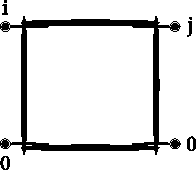
\includegraphics{immagini/circbase.pdf}}
 \hspace{25pt}
 \subfloat[Circuito modificato]{\label{fig:circmod}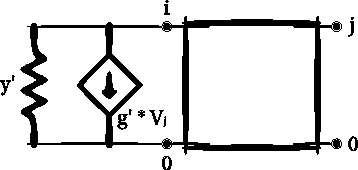
\includegraphics{immagini/circmod.pdf}}
 \caption{Metodo del circuito modificato}
 \label{fig:circmet}
\end{figure}

Sebbene il calcolo illustrato sia a tutti gli effetti corretto, non si può dire che sia allo stesso tempo anche efficace e maneggevole. Qui entra in gioco il metodo del circuito modificato, atto a rendere facilmente recuperabili i dati sensibili coinvolti nell'analisi.

In figura \ref{fig:circmet} è riportato visivamente ciò di cui consiste concretamente questa tecnica. Rifacendosi all'esempio sopra citato, cioè ad una sollecitazione applicata fra i nodi $i$ e $0$ per poi valutarne gli effetti sui terminali $j$ e $0$, si può guardare al circuito come nella forma proposta in figura \ref{fig:circbase}. Aggiungendo quindi fra i due nodi in ingresso un'ammettenza e una transcoduttanza\graffito{Ammettenza e transconduttanza ausiliarie introdurranno nei due grafi archi che dovranno essere marcati con speciali valori per quanto riguarda la loro tipologia, pur rientrando nella categoria delle ammettenze}, quest'ultima legata ai terminali di uscita, si ricava il circuito modificato riportato in figura \ref{fig:circmod}. Il determinante della matrice delle ammettenze per il circuito modificato diventa:
$$ \Delta ' = \Delta + y'\Delta_{ii} + g'\Delta_{ij} $$
Si nota come siano stati di fatto ricavati in modo immediato i cofattori coinvolti nel calcolo dell'impedenza in ingresso, la transimpedenza e la funzione di trasferimento. Sarà adesso possibile procedere senza difficoltà ricercando in $\Delta '$ tutti i valori d'interesse, semplicemente individuando $y'$ e $g'$.

\chapter{Esempio: divisore di tensione}

\begin{figure}
 \centering
 \subfloat[Divisore di tensione]{\label{fig:resol}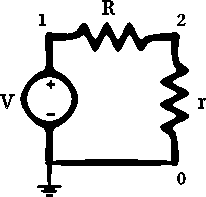
\includegraphics[scale=0.90]{immagini/resol.pdf}}\hspace{50pt}
 \subfloat[Modello dipendente]{\label{fig:resoldip}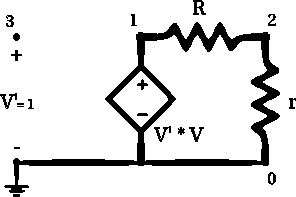
\includegraphics[scale=0.90]{immagini/resoldip.pdf}}\\\vspace{20pt}
 \subfloat[Modello equivalente]{\label{fig:resoleq}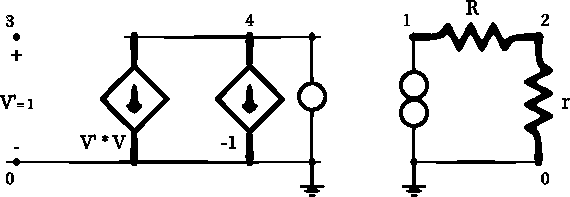
\includegraphics[scale=0.90]{immagini/resoleq.pdf}}\\\vspace{20pt}
 \subfloat[Circuito modificato]{\label{fig:resolmod}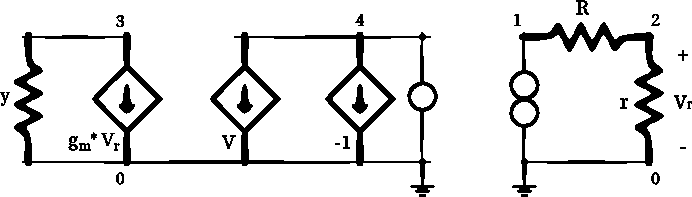
\includegraphics[scale=0.90]{immagini/resolmod.pdf}}\\\vspace{20pt}
 \subfloat[Grafi in corrente (G.I.) e in tensione (G.V.)]{\label{fig:resolgs}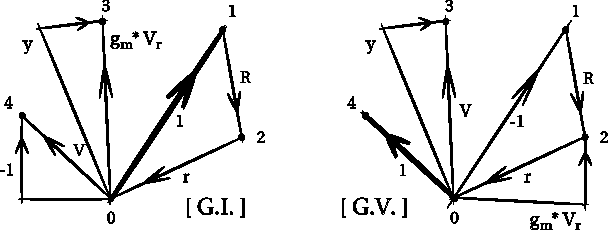
\includegraphics{immagini/resolgs.pdf}}
 \caption{Analisi successiva per il divisore di tensione}
 \label{fig:resolall}
\end{figure}

Per terminare questa parte, sfruttando la teoria esposta fino ad ora, viene proposto un esempio di analisi simbolica, dal disegno fino alle fasi di risoluzione per un semplice circuito. Dall'esempio si potrà osservare come anche una rete elementare finisca col trasformarsi, attraverso mutazioni e adattamenti successivi, in una struttura equivalente ben più complessa ma risolvibile. Non deve spaventare il fatto che un semplice circuito composto da tre componenti si traduca, alla fine, in una rete contenente tre resistenze, tre generatori controllati e un nullore (cioè una coppia nullatore-noratore), poiché questo altro non è che l'inevitabile risultato dell'applicazione delle tecniche precedentemente esposte.

Le varie fasi attraversate sono riportate in successione in figura \ref{fig:resolall}. Nella \ref{fig:resol} si ha il circuito che si vuole analizzare, un semplice divisore di tensione composto di un generatore di tensione e due resistenze; un totale di tre nodi è richiesto dall'utente per il disegno, è noto però che questa quantità lieviterà a causa della richiesta di nodi fittizi messa in atto da specifici componenti.

In figura \ref{fig:resoldip} si opera la prima modifica, ovvero si attua la sostituzione del generatore di tensione rendendo di fatto quello presente nel circuito sottomesso un generatore di tensione controllato in tensione. Questo è possibile per il fatto che durante le fasi di risoluzione si considera come generatore unico interno al circuito un componente fittizio ininfluente da cui tutti gli altri dipenderanno (ovvero, i generatori di corrente e di tensione diventeranno a loro volta generatori controllati in tensione dall'elemento fittizio). Col termine ininfluente si indica il fatto che esso è trattato come elemento non simbolico e ha valore unitario, per cui sistemando in modo corretto i parametri coinvolti non influisce affatto sul risultato finale. Dall'immagine si può notare come, appunto, la tensione ottenuta attraverso il generatore controllato abbia di fatto valore identico a quella proposta nel circuito originale.

In figura \ref{fig:resoleq} viene fatto un ulteriore passo avanti, avviene cioè la sostituzione del generatore controllato precedentemente inserito col suo modello equivalente, composto da generatori di corrente controllati in tensione e nullori. Se già al passo precedente il numero di nodi richiesti era aumentato, un'ulteriore crescita si ha in questa sede, portando il totale a cinque nodi e ritrovandosi con un circuito ben lungi dall'assomigliare all'originale proposto. Ancora, sebbene possano risultare difficilmente comprensibili i valori associati ai diversi elementi coinvolti durante la sostituzione, rifacendosi ai capitoli precedenti si ha che vale per il generatore di tensione controllato in tensione, dal modello equivalente (dove $g$ e $g'$ siano i parametri dei generatori di corrente controllati in tensione):
$$ V_{out} = -\frac{g}{g'}\ast V_{in};\quad I_ {in} = 0; $$
Per cui per $V_{in}$ unitario, posto $g'$ pari a $-1$, si può modellare $g$ a piacimento così da ottenere il valore desiderato per $V_{out}$. Nel caso specifico, $g$ ha assunto il valore associato al generatore indipendente presente nel circuito originale.

Procedendo, nella \ref{fig:resolmod} viene illustrato come risulta la rete una volta modificata, ovvero una volta aggiunta la circuiteria d'ingresso. Questa, ricordiamo, è utile allo scopo di rendere facilmente estrapolabile, dal computo finale dell'equazione, l'insieme di elementi che andranno a costituire numeratore e denominatore della funzione d'uscita. Il circuito finalmente modificato e rielaborato secondo le necessarie sostituzioni, si presenta nella sua forma finale e può essere sottoposto al risolutore vero e proprio che si aspetta, appunto, un particolare tipo di reti composte solo ed esclusivamente da specifici componenti (tutti quelli che è in grado realmente di trattare).

\paragraph{}

L'operazione successiva consiste nello spostarsi dallo spazio dei circuiti elettrici in quello dei grafi\graffito{Dovrebbe far riflettere l'idea che il problema attraversa orizzontalmente aree tematiche diverse, spogliandosi del suo significato originario e andando a trovare una soluzione concreta altrove, per poi adottarla nel contesto di partenza}, attraverso una traduzione componente per componente della rete finale ottenuta. In figura \ref{fig:resolgs} sono riportati i due grafi in tensione e in corrente ottenuti da questo processo, evidenziando in grassetto gli archi dovuti al nullore (che, sottolineiamo, devono essere forzati in ogni albero di copertura comune) e quello che si potrebbe definire il peso del singolo arco, ovvero il valore ad esso associato (in questo esempio si assume, senza perdita di generalità, un'analisi prettamente simbolica). Sui due grafi così ottenuti non resta che applicare l'algoritmo di ricerca degli alberi di copertura comuni, il quale restituirà i seguenti elenchi di archi (indicati col peso associato per essere distinti, laddove ve ne siano più d'uno fra una stessa coppia di nodi):
\begin{enumerate}
 \item $ \left[\; 1,\; y,\; -1,\; R\;\right] $
 \item $ \left[\; 1,\; y,\; -1,\; r\;\right] $
 \item $ \left[\; 1,\; g_m * V_r,\; V,\; R\;\right] $
\end{enumerate}
Ovviamente, avendo cinque nodi, gli alberi sono composti da quattro archi ognuno. Tralasciando il calcolo del parametro $\varepsilon_i$, il quale procedimento si descrive come la mera riduzione della matrice d'incidenza associata ai singoli alberi e quindi al calcolo del determinante di detta matrice, si nota fin da subito come da quanto ottenuto si possano ricavare immediatamente i dati necessari al calcolo dell'espressione finale. Seguendo infatti l'ordine degli alberi sopra riportati e considerando l'approccio di scelta delle ammettenze sull'albero e delle impedenze sul coalbero, oltre che rifacendosi al fatto illustrato per cui gli alberi comprendenti il ramo $y$ vanno al denominatore e gli alberi contenenti il ramo $g_m * V_r$ vanno al numeratore, abbiamo quanto segue:
\begin{enumerate}
 \item Nessuna ammettenza sull'albero, impedenza $r$ sul coalbero.
 \item Nessuna ammettenza sull'albero, impedenza $R$ sul coalbero.
 \item Ammettenza $V$ sull'albero (nota: $V$ è un valore dovuto alla presenza del generatore di corrente controllato in tensione, da cui il suo ruolo come ammettenza), impedenza $r$ sul coalbero.
\end{enumerate}
Bisogna fare una precisazione sui rami $y$ e $g_m$. Nella pratica, anche laddove essi rechino dati significativi, bisogna interpretarli solo ed esclusivamente come marcatori per quegli alberi che andranno a comporre l'equazione finale. Pertanto, nonostante almeno uno di essi potrebbe dare il suo apporto in questa fase, una volta individuati ed estratti gli alberi da essi indicati, sono di fatto esclusi da ogni fase successiva e con loro il carico informativo trasportato.

Arrivati a questo punto, poiché la regola impone che si moltiplichino componenti di uno stesso albero e si sommino elementi su alberi differenti, si ricava come atteso:
$$ \frac{V * r}{R + r} $$

\paragraph{}

Inutile dire che il procedimento sopra descritto in maniera esaustiva e particolareggiata può essere snellito e migliorato sotto diversi aspetti e, nella realtà, discosta abbastanza da quello illustrato pur rimanendo fedele ai principi e alle linee guida che hanno pilotato l'illustrazione. Di fatto, per esempio, l'introduzione di un generatore globale fittizio da cui tutti vengano a dipendere è una richiesta che si scontra con le necessità di ridurre i tempi di calcolo, pertanto si può usare il primo generatore incontrato durante la sintesi ponendolo come globale e facendo dipendere da esso tutti i successivi. Allo stesso modo sarà inutile sostituire sorgenti indipendenti con sorgenti controllate, quindi quest'ultime con modelli equivalenti, quando in un unico passo si può applicare la trasformazione diretta saltando la fase intermedia.

Queste sono soltanto alcune delle tante possibilità di ottimizzazione della procedura messe in atto durante lo sviluppo vero e proprio.



\cleardoublepage
\part{\ldots alla Pratica}

\thispagestyle{empty}
\null\vspace{\stretch{1}}
\begin{flushright}
\setlength{\epigraphwidth}{21em}
\epigraph{
\footnotesize{''Quarantadue!'' $[[$\ldots$]]$ ''Questo è tutto ciò che sai dire dopo un lavoro di sette milioni e mezzo di anni{?}``}
}{\footnotesize{Guida galattica per autostoppisti\\ Douglas Adams}}
\end{flushright}\vspace{\stretch{2}}\null

\chapter{Framework}

Lo sviluppo del software QSapecNG si è appoggiato a framework esistenti, in grado di offrire tutto ciò che fosse necessario per snellire, semplificare ed ottimizzare la procedura di scrittura del codice. In particolare, data la crucialità del ruolo ricoperto dall'algoritmo per la ricerca degli alberi di copertura comuni su due grafi, era necessario appoggiarsi ad una libreria che mettesse a disposizione allo stesso tempo strutture dati maneggevoli per la definizione di grafi e modelli flessibili per la stesura di algoritmi che operassero su tali grafi. Non meno importante si è dimostrata anche la necessità di disporre di una libreria di componenti grafici capace di dimostrarsi completa sotto tutti gli aspetti e in grado di rendere veloce lo sviluppo senza appesantirlo in un crescendo di complessità. Non bisogna poi tralasciare tutti quegli aspetti che all'utente finale possono apparire come di corredo o addirittura essere celati ma che, nelle fasi di sviluppo, possono presentarsi come veri e propri ostacoli e per questo motivo devono essere affrontati con i giusti mezzi.

Per tutti i motivi sopra brevemente accennati e per molti altri che sarebbe tedioso elencare, la scelta è ricaduta su due pietre miliari del mondo C++, ovvero:
\begin{itemize}
 \item La libreria di librerie C++: Boost C++ Libraries \cite{Boost}.
 \item Il framework Qt \cite{Qt}, componenti per lo sviluppo di applicativi multi-piattaforma grafici e non.
\end{itemize}
Grazie ad esse il software QSapecNG si è sviluppato in modo pulito e coerente, con un po' di oculatezza nella scrittura è risultato essere interamente portabile e pertanto si presenta come un applicativo multi-piattaforma per il disegno, la risoluzione simbolica e l'analisi del comportamento di circuiti elettrici.\\
Senza dilungarsi troppo, è necessario quindi effettuare una veloce panoramica dei due colossi utilizzati.


\section{Boost C++ Libraries}
Da Herb Sutter e Andrei Alexandrescu viene definita \cite{CppCodStd} come:
\begin{quote}
 ... one of the most highly regarded and expertly designed C++ library projects in the world.
\end{quote}

Scott Meyers avanza un consiglio in proposito \cite{EffectiveCpp} fra le cose da fare per i novizi del pianeta C++:
\begin{quote}
 Item $55$: Familiarize yourself with Boost.
\end{quote}

Bjarne Stroustrup, una delle menti che stanno dietro alla definizione del linguaggio C++ e autore del libro \cite{Stroustrup} considerato la guida introduttiva di base per chi vuole avvicinarsi al linguaggio, alla domanda su cosa pensi di Boost risponde:
\begin{quote}
Boost is a large and expanding collection of libraries designed to work well with the ISO C++ standard library. It contains many extremely useful and well-engineered libraries, such as asio, filesystem, regex, and thread (apologies for not trying to identify more useful libraries; there are just too many). One library, $TR1$, contains a good approximation of new C++$0x$ standard library components.

The Boost libraries
\begin{itemize}
 \item Have tests suites.
 \item Have documentation.
 \item  Have been tested on multiple systems.
 \item Are peer-reviewed.
\end{itemize}

[...]

That said, it is usually a really dumb idea to go and reinvent a wheel that boost already offers.
\end{quote}
Mentre in un suo articolo \cite{StroustrupCpp} afferma:
\begin{quote}
 The obvious solution for most programmers is to use a library that provides an elegant and efficient platform independent to needed services. Examples are BOOST...
\end{quote}

Boost C++\graffito{Boost C++ è spesso usata come ausilio alla programmazione, per sopperire a tutte le carenze della libreria standard (plausibili, motivate o meno)}, quella che si potrebbe definire una libreria di librerie risulta quindi essere apprezzata e ben vista anche dai maggiori esponenti dell'ambiente C++, al di là del suo essere equilibratamente complicata tanto per i novizi quanto per gli esperti. Sviluppata in maniera modulare e con componenti strettamente legati l'un l'altro (croce e delizia di chi si avvicina per la prima volta), offre alti standard di qualità e un ventaglio di soluzioni per le più disparate necessità. Si articola attraverso tecniche di programmazione generica, l'uso di \textit{concept} e \textit{traits} e molto altro ancora, mostrandosi in grado di rendere estremamente flessibile lo sviluppo e l'utilizzo delle diverse librerie, alzando soltanto di poco la curva di apprendimento e mettendo a disposizione in molti casi soluzioni semplici per chi preferisce non scoprire cosa vi è dietro.

Le librerie Boost C++ sono di fatto, volenti o nolenti, una realtà sempre più integrata negli standard C++ che da essa attingono e ad essa forniscono gli strumenti per migliorarsi sempre più. Una realtà che, inevitabilmente, deve essere presa in considerazione e spesso offre la risposte a gran parte delle problematiche incontrate nello sviluppo.

\paragraph{BGL: The Boost Graph Library}
Sarebbe interessante, in questo frangente, discutere di tutte le librerie presenti in Boost e utilizzate anche nella stesura del codice di QSapecNG (quali \textit{Property Tree}, \textit{Property Map}, \textit{Foreach}, \textit{Bimap} e via dicendo), eppure un tale argomento risulterebbe forse fin troppo ampio e mal digerito da chiunque non sia appassionato di programmazione e interessato ai dettagli del software.\\
Ciò nonostante bisogna obbligatoriamente soffermarsi almeno su una di esse, poiché si sono sviluppati algoritmi conformi alle direttive proposte che vanno a collocarsi direttamente nella panoramica offerta da Boost. Un'analisi dettagliata di tali algoritmi è riportata nei capitoli che seguono mentre una breve introduzione e descrizione della libreria interessata avrà qui luogo.

In particolare la libreria in questione è la \textbf{BGL: Boost Graph Library} \cite{BGL}. Essa rappresenta una risposta alla necessità di strutture dati per la rappresentazione e gestione di grafi, oltre a fornire le basi per lo sviluppo di codice generico da applicare su tali strutture (nel caso specifico, atto ad individuare gli alberi di copertura comuni dati due grafi).\\
La BGL mette a disposizione interfacce, algoritmi e componenti generici nello stesso senso in cui risulta generica la \textbf{STL (Standard Template Library)} \cite{STL}. Come riportato dalla documentazione, la BGL è generica nei modi che seguono (parafrasando appunto il modello della STL):
\begin{itemize}
 \item Interoperabilità fra algoritmi e strutture dati: i grafi sono sviluppati su un concetto di interfaccia e nascondono la reale implementazione (sia essa in forma di lista di archi, matrice o lista di adiacenza), per cui gli algoritmi possono essere resi altrettanto generici e trattare svariati tipi di grafi, accedendo attraverso iteratori su archi e vertici in modo coerente ed omogeneo, senza preoccuparsi della forma e struttura sottoposta in ingresso.
 \item Estensione degli algoritmi: l'uso di oggetti conformi ad una interfaccia comune, detta visitatore, permette di estendere facilmente tutti quegli algoritmi a cui tali interfacce possono essere agganciate per dare luogo ad azioni specifiche in ben definiti punti chiave dell'esecuzione.
 \item Multi-parametrizzazione delle proprietà per vertici ed archi: senza scendere in dettagli, poiché l'argomento richiederebbe l'introduzione di un'ulteriore libreria presente in Boost (\textit{Property Map}), basti sapere che archi e vertici possono essere associati ad un numero arbitrario e indipendente di proprietà, ovvero informazioni che recano con loro durante l'esecuzione.
\end{itemize}

Inutile dire, poi, che è già disponibile un ampio parco di algoritmi base\graffito{Alcuni degli algoritmi presenti nella BGL sono la ricerca in profondità (depth first search, DFS), la ricerca in ampiezza (breadth first search, BFS), la ricerca del cammino minimo (algoritmo di Dijkstra), la ricerca delle componenti connesse e fortemente connesse, e molti altri ancora, alcuni dei quali proposti in più forme (ad esempio l'algoritmo per la ricerca degli alberi di copertura a peso minimo è presente nella versione di Kruskal e in quella di Prim)} da usare come tasselli per la costruzione di funzioni più complesse, anch'esse presenti per quanto possibile. Bisogna dire che non è disponibile, forse a causa della specificità dell'argomento, un algoritmo per la ricerca di alberi di copertura comuni fra due grafi, il quale sarà presto e orgogliosamente proposto (proprio a seguito dello sviluppo nell'ottica di QSapecNG) per l'integrazione nella BGL, essendo anche questo uno dei risultati ottenuti durante il lavoro di tesi.


\section{Qt}

\begin{figure}
 \centering
 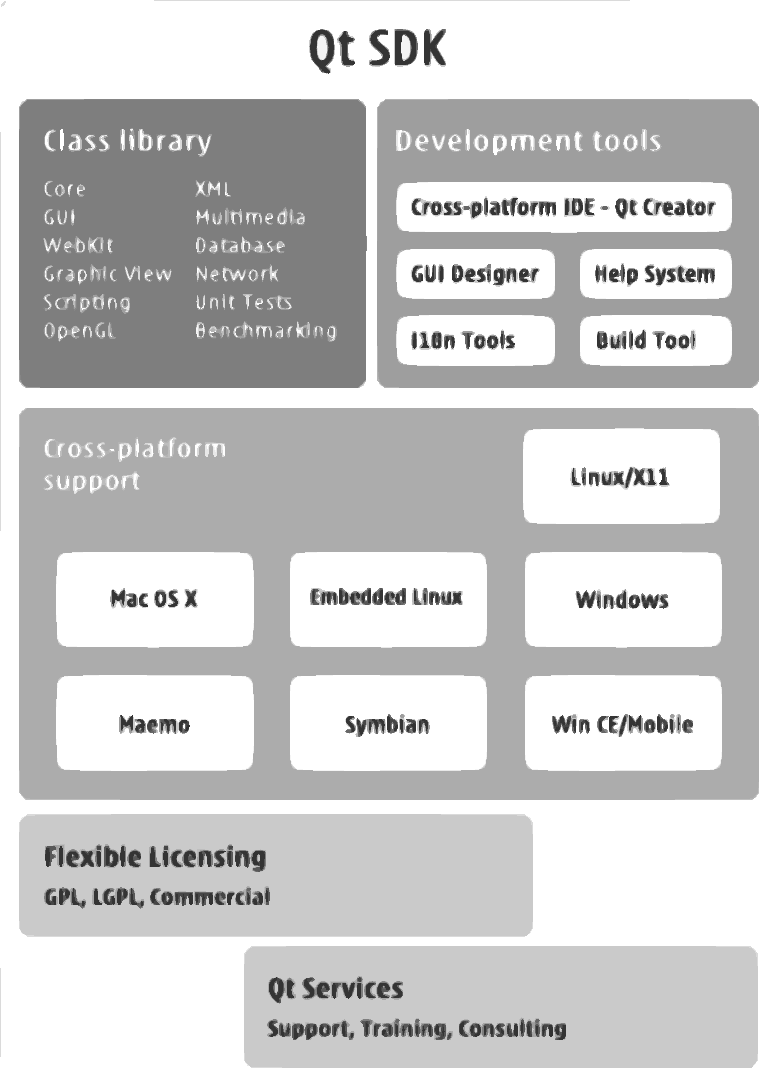
\includegraphics[scale=0.85]{immagini/qtschema.pdf}
 \caption{Qt SDK (schema)}
 \label{fig:qtschema}
\end{figure}

L'ambiente grafico (e non solo) ha sposato, invece, la proposta delle librerie Qt \cite{Qt}, un framework che non si limita ad offrire componenti per lo sviluppo di interfacce ma mette a disposizione molto di più, come ad esempio la possibilità di fornire soluzioni portabili, multi-threading, accessibili via web e tanto altro ancora.

Il Qt SDK (Software Development Kit), in figura \ref{fig:qtschema}, non rappresenta un semplice strumento o una libreria, è tutto ciò (o quasi) di cui uno sviluppatore può avere bisogno: librerie per lo sviluppo grafico, per il web, per il multimediale, per le basi dati e tanto altro a supporto delle necessità del programmatore; strumenti di sviluppo quali un IDE (Integrated Development Environment) multi-piattaforma, un ambiente per il disegno diretto delle interfacce, un sistema per la traduzione agile in lingue diverse rappresentano la punta dell'iceberg di offerte che accompagnano il framework; il modello di licenza, i servizi (gratuiti e non) messi a disposizione e il pieno supporto su un'ampia varietà di piattaforme sono il biglietto da visita del Qt SDK.

Anche in questa sede sarebbe forse interessante scendere dettagliatamente nel cuore del come e del cosa riguardanti lo sviluppo di un sistema CAD ma purtroppo, per ovvi motivi, questo non è realmente possibile. Più avanti saranno però trattati alcuni pattern che da Qt migrano direttamente nel processo di progettazione del software che fa uso di queste librerie, cercando di dare un'idea introduttiva sulle metodologie di programmazione utilizzate.

\chapter{Software Design}

In questo capitolo sono discussi alcuni degli spunti più interessanti e delle soluzioni più ingegnose adottate durante lo sviluppo del software QSapecNG. Viene inoltre illustrata e per quanto possibile descritta nei particolari la procedura generica di ricerca degli alberi di copertura comuni fra due grafi, proposta secondo il modello introdotto da Boost C++ e sottoposta proprio a quest'ultima (all'attenzione della BGL) per l'integrazione.

Per ovvi motivi non è possibile trattare per intero il codice scritto, poiché questo richiederebbe probabilmente svariati capitoli a sé dedicati per essere analizzato nei dettagli e per visitare tutte le relazioni che legano fra loro le diverse parti. Ad ogni modo, nei capitoli che seguiranno sarà discusso l'orientamento adottato durante lo sviluppo, atto a rendere migliorabile e a dare un più ampio respiro al software.


\section{MRT: Tecniche di Programmazione Generica}

Come già anticipato, Boost C++ in primis e quindi la BGL a seguire adottano una metodologia di programmazione generica\graffito{La programmazione generica è uno dei punti cardine del C++ in genere e Boost C++ ne fa uno dei suoi punti di forza, sfruttandone totalmente le potenzialità} con lo scopo di rendere quanto più flessibili tanto le strutture dati quanto gli algoritmi su di esse applicabili. Chi critica Boost C++ prende proprio questo argomento, da cui deriva un aumento di pesantezza in fase di compilazione e un più alto grado di difficoltà d'uso in fase di sviluppo e di partecipazione, come arma per attaccare la libreria. Di contro, però, negli anni la scelta ha ripagato i suoi padri e anche in un modesto lavoro di tesi si è potuto godere dei vantaggi dati, oltre che apportare il proprio contributo.

Allo scopo di aiutare la comprensione di quanto seguirà, è necessario introdurre brevemente alcuni di questi concetti.

\paragraph{Concept} I \textit{concept} rappresentano, detto in parole povere, un meccanismo di controllo sulla conformità di determinati oggetti rispetto a determinati requisiti. Per capirne l'utilità conviene inquadrarli in uno dei loro ambiti d'uso più comune, ovvero i \textit{template}. Quest'ultimi sono sviluppati su un'idea di tipo di dato astratto, sul quale operano, eppure il C++ non fornisce in alcun modo un meccanismo per verificare che il dato sottomesso come parametro sia effettivamente valido (sia cioè un modello per il concetto astratto).\graffito{La peculiarità dei concept è quella di essere composti da codice che in fase di compilazione permette di controllare il rispetto del concetto vero e proprio, mentre all'invocazione del linker viene scartato da quest'ultimo poiché risulta essere non effettivamente utilizzato, pertanto non contribuisce in alcun modo ad appesantire il prodotto finale} Questo può portare a indicazioni hard-coded all'interno dei template stessi o a nomi fantasiosi, che però vengono ignorati dal compilatore (ai fini della compilazione, RandomAccessIterator non è differente da T come nome di parametro). Questo si traduce in:
\begin{itemize}
 \item Errori criptici in fase di compilazione che possono essere forse facilmente decifrabili per un programmatore esperto ma non per chi si è da poco avvicinato al linguaggio.
 \item Mancanza di documentazione o errori sulle specifiche esatte richieste per la conformità di un modello al concetto.
 \item Possibilità che richieste formali in forma di commento risultino difficili da esprimere, con il rischio di diventare troppo blande o più stringenti di quanto non sia realmente necessario.
 \item Concetti documentati nel codice e documentazione per utente finale potrebbero essere discordanti, disorientando quest'ultimo.
\end{itemize}
In questo panorama si collocano pertanto i concept,\graffito{Di fatto i concept forzano una classe ad essere almeno conforme ad una specifica interfaccia, attraverso la quale verrà acceduta} con lo scopo di semplificare la procedura, rendere espliciti i requisiti, rendere maggiormente comprensibili eventuali messaggi di errore e aiutare nel complesso tanto lo sviluppatore quanto l'utente dei template che ne fanno uso (siano essi strutture dati o funzioni generiche, indifferentemente).

\paragraph{Traits} I \textit{traits} rappresentano una delle più importanti tecniche di programmazione generica in C++ e sono ampiamente usati all'interno di Boost C++. Essi permettono di prendere decisioni basate sui tipi in fase di compilazione, così come strutture quali l'\textit{if} permettono di prendere decisioni basate su valori in fase di esecuzione. Per questo motivo i traits vengono spesso chiamati l'\textbf{if-then-else} dei tipi. Essi sono non intrusivi e permettono di associare informazioni ad entità in fase di compilazione.

\paragraph{Tag Dispatching} Questa è una tecnica per sfruttare l'overloading delle funzioni allo scopo di mutarne il comportamento basandosi sulle proprietà di un tipo, letteralmente smistare le richieste fra le diverse funzioni sulla base del tipo fornito come proprietà. Sono spesso usati in concomitanza con l'uso dei traits poiché le proprietà atte allo smistamento sono solitamente accessibili attraverso la tecnica dei traits.

\paragraph{}
Questi sono soltanto alcuni dei principi alla base della programmazione generica, come interpretata in Boost C++. Eppure sono utili poiché rappresentano quei principi la cui comprensione risulterà necessaria per approfondire la discussione dell'algoritmo di ricerca per gli alberi di copertura comuni a due grafi. Ciò nonostante, per chi fosse interessato nei dettagli della singola istruzione, sia chiaro che non è questa la sede per illustrare la logica che sta dietro alle scelte fatte e probabilmente richiederebbe non poco spazio l'affrontare un'analisi dettagliata di un algoritmo, anche semplice, appartenente o proposto per la BGL.

\paragraph{}

\begin{lstlisting}[basicstyle=\small,language=C++,caption={Parte della funzione \textit{mrt}},float,captionpos=b,label={lst:mrtstub},frame=lines,numbers=left]
template <
  class Graph, class Order, class Func, class Seq >
BOOST_CONCEPT_REQUIRES(
  ((RandomAccessContainer<Order>))
  ((IncidenceGraphConcept<Graph>))
  ((UnaryFunction<Func, void, Seq>))
  ((Mutable_RandomAccessContainer<Seq>))
  ((VertexAndEdgeListGraphConcept<Graph>)),
  (void))
mrt_two_graphs_common_spanning_trees
  ( const Graph& iG, Order iG_map,
    const Graph& vG, Order vG_map,
    Func func, Seq inL )
{
  typedef graph_traits<Graph> GraphTraits;

  typedef typename GraphTraits::directed_category directed_category;

  // [...]

  typedef typename GraphTraits::edge_descriptor edge_descriptor;
  typedef typename GraphTraits::edges_size_type edges_size_type;

  // [...]

  typedef typename Seq::value_type seq_value_type;
  typedef typename Seq::size_type seq_size_type;

  // [...]

  typedef typename Order::value_type order_value_type;
  typedef typename Order::size_type order_size_type;

  // [...]

  BOOST_STATIC_ASSERT((is_same<order_value_type, edge_descriptor>::value));
  BOOST_CONCEPT_ASSERT((Convertible<order_size_type, edges_size_type>));
  BOOST_CONCEPT_ASSERT((Convertible<seq_size_type, edges_size_type>));
  BOOST_STATIC_ASSERT((is_same<seq_value_type, bool>::value));
  BOOST_STATIC_ASSERT((is_same<directed_category, undirected_tag>::value));

  // [...]
}
\end{lstlisting}

  Per cominciare, rifacendosi subito ad alcuni dei punti sopra esposti, è molto interessante studiare la parte introduttiva della funzione di ricerca per gli alberi comuni fra due grafi, riportata (opportunamente ripulita dal superfluo per motivi di spazio) nel listato \ref{lst:mrtstub}. Probabilmente all'apparenza piuttosto complessa, tralasciando le dichiarazioni di MACRO prettamente legate a Boost C++, è facilmente interpretabile ed esplicita nelle intenzioni. Inoltre è sufficiente comprendere come essa debba essere invocata, senza dilungarsi sull'effettiva implementazione, per capire un po' meglio l'importanza e l'utilità delle tecniche di sviluppo adottate.\\
  In questo frangente è necessaria una nota: questa non è l'unica chiamata disponibile per la funzione, bensì la più completa. Esistono altre interfacce utilizzabili da chi non voglia sottomettere un ordine (viene usato quello estraibile direttamente dai grafi stessi) o per chi non intenda usufruire degli alberi individuati, sebbene questo abbia di per sé poca utilità ai fini pratici.

\begin{figure}[t]
 \centering
 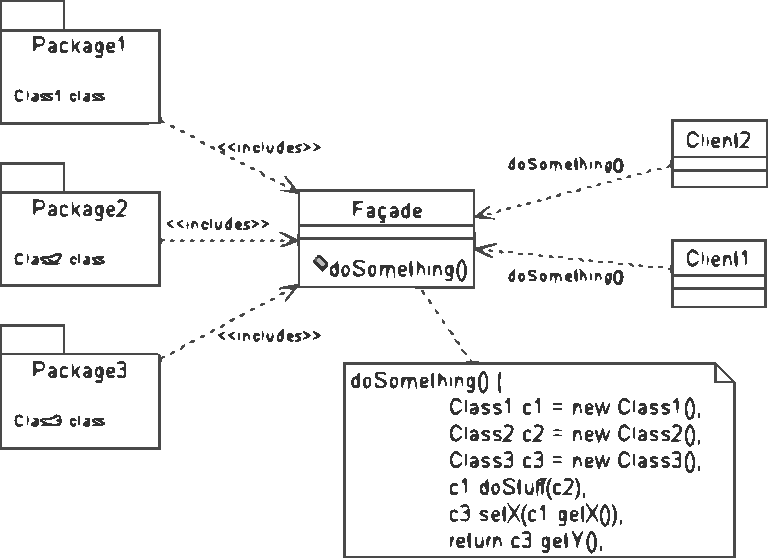
\includegraphics[scale=0.80]{immagini/facade.pdf}
 \caption{Pattern Facade, modello per la funzione \textit{mrt}}
 \label{fig:facade}
\end{figure}

La funzione \textit{mrt} rappresenta il punto di ingresso per un labirinto ben più articolato di strutture dati e chiamate a funzione, celato all'utente finale e accessibile attraverso una semplice chiamata ad essa. Rifacendosi al pattern \textit{Facade},\graffito{Il pattern Facade è molto importante, poiché permette di celare dietro un'amichevole chiamata di funzione la complessità di una serie di operazioni che risulterebbero estremamente complesse nel loro utilizzo se lasciate all'utente} riportato in figura \ref{fig:facade}, questa funzione nasconde al suo interno l'approccio ricorsivo dell'algoritmo e tutte quelle richieste e definizioni di strutture necessarie all'espletamento dei propri compiti.

Come si nota ad una prima occhiata, essa sfrutta le possibilità offerte dalla programmazione generica e richiede di essere parametrizzata su:
\begin{itemize}
 \item Un modello di grafo, \textit{Graph}, a cui i due grafi sottomessi su cui effettuare la ricerca dovranno essere conformi.
 \item Un modello di ordine, \textit{Order}, ovvero una struttura atta all'utilizzo per l'interrogazione relativa all'indice associato ai singoli archi.
 \item Un modello di funzione, \textit{Func}, utilizzata prevalentemente per l'invocazione su ogni albero individuato.
 \item Un modello di contenitore, \textit{Seq}, per immagazzinare gli archi via via che vengono inseriti nei potenziali alberi.
\end{itemize}
Sebbene al momento possano risultare abbastanza oscuri i veri utilizzi di questi oggetti, saranno chiari a breve, ovvero una volta osservati i concetti a cui devono rifarsi. Seguendo lo stesso ordine di cui sopra, studiando meglio il tutto:
\begin{itemize}
 \item Per quanto riguarda Graph, le prime cose da osservare sono due dichiarazioni che ne definiscono completamente la struttura, ovvero:
   \begin{enumerate}
    \item La necessità che esso sia conforme al concetto (definito dalla BGL stessa) di \textit{IncidenceGraph} (riga 5), un'interfaccia che permette un accesso efficiente per gli archi in uscita dal singolo vertice.
    \item La necessità che esso sia conforme al concetto (definito dalla BGL stessa) di \textit{VertexAndEdgeListGraph} (riga 8), il quale permette l'attraversamento di tutti i vertici e l'accesso a tutti gli archi in modo semplice ed immediato.
   \end{enumerate}
 Queste richieste sono legate anche e non solo agli algoritmi base utilizzati, già presenti nella BGL e quindi non re-implementati, e ai loro vincoli di concetto. Meno interessanti le definizioni che seguono, molte delle quali saranno discusse anche nei punti seguenti poiché relative pure ad altri elementi. Da sottolineare la presenza (riga 40) dell'imposizione sul fatto che il grafo sia non orientato: questo è necessario per i motivi già esposti nei capitoli precedenti, poiché permette un corretto accesso al grafo e non esclude il fatto che si possa conoscere l'effettivo orientamento del singolo arco attraverso la sua definizione, che porta con sé intrinsecamente tale informazione. Ancora, da notare come quest'ultimo particolare sia alla base del \textit{tag dispatching}.
 \item La prima dichiarazione pilota il modello Order (riga 4), affermando che esso deve essere conforme a quello di un contenitore ad accesso causale, come definito in \cite{STL}. Banalmente questo dovrebbe far subito intuire che la volontà è quella di rendere Order un contenitore di tipo vettore a cui si accede tramite la definizione di un arco, ottenendone l'indice associato (o meglio, accedendo con l'$i_{esimo}$ indice si ricava l'arco associato, che rappresenta poi in realtà la soluzione effettivamente adottata in QSapecNG nella forma di un vettore). Proseguendo infatti nello studio delle definizioni associate ad Order si ha che, a seguito di una ridenominazione delle informazioni contenute (righe 31-32, per semplicità d'uso), viene accertata l'equivalenza fra il tipo dati contenuti e quello che descrive effettivamente un arco e quindi verificata la convertibilità fra le tipologie di indicizzazione nei due spazi (righe 36-37).
 \item Come detto parlando a proposito di Func, questo oggetto rappresenta il prototipo di una funzione a cui verranno sottomessi gli alberi di copertura comuni, una volta individuati. Poiché Seq è destinato a contenere gli archi di tali alberi prima, durante e a costruzione finita, Func riceverà in ingresso proprio tale lista (riga 6) restituendo niente in uscita. Questo è, di fatto, sufficiente a descrivere completamente l'oggetto Func, delegando agli altri elementi tutto il resto (tipo di archi, di indici, etc.).
 \item Ultimo ma non meno importante è Seq, che rappresenta un contenitore per mantenere gli archi dell'albero di copertura comune ai due grafi durante la ricerca (ovvero, la costruzione). In particolare (riga 7) viene richiesto che, come già successo per Order, esso sia definito come un contenitore ad accesso causale ma con la particolarità di essere modificabile (intuitivamente è destinato ad un uso di inserimento e rimozione di elementi al suo interno o di modifica di quest'ultimi). Procedendo, però, si ricavano informazioni in grado di chiarire il vero scopo di Seq (righe 38-39). Viene infatti verificata la convertibilità dei suoi indici di accesso con quelli che permettono di accedere agli archi all'interno di un grafo, ma ancora più importante viene imposto che il tipo di dato contenuto sia una variabile booleana. Se fosse stato riportato uno spezzone maggiore di software, si sarebbe potuto notare anche la verifica in codice sulla stessa dimensione dei due spazi (ovvero sul fatto che i componenti contenuti in Seq fossero in numero pari agli archi da analizzare). Riassumendo: a partire dagli elementi ottenuti, quindi, si deduce che Seq potrà essere ad esempio rappresentato da un vettore di dimensione pari al numero di archi nei due grafi e contenente variabili booleane, le quali indicano la presenza (\textbf{true}) o meno (\textbf{false}) dell'$i_{esimo}$ arco all'interno del $j_{esimo}$ albero.
\end{itemize}

Con queste poche nozioni si riesce a modellare in maniera sufficientemente facile un ambiente in grado di istanziare, inizializzare e sottomettere i corretti oggetti alla funzione di ricerca per gli alberi comuni fra due grafi. Il resto del codice si riduce a mere chiamate alle funzioni fornite dalla BGL che ricalcano fedelmente l'algoritmo esposto nei capitoli precedenti e non è pertanto di pari interesse.

\paragraph{}

\begin{lstlisting}[basicstyle=\small,language=C++,caption={Tree Collector},float,captionpos=b,label={lst:treecoll},frame=lines,numbers=left]
template <class Coll, class Seq>
struct tree_collector
{

public:
  BOOST_CONCEPT_ASSERT((BackInsertionSequence<Coll>));
  BOOST_CONCEPT_ASSERT((RandomAccessContainer<Seq>));
  BOOST_CONCEPT_ASSERT((CopyConstructible<Seq>));

  typedef typename Coll::value_type coll_value_type;
  typedef typename Seq::value_type seq_value_type;

  BOOST_STATIC_ASSERT((is_same<coll_value_type, Seq>::value));
  BOOST_STATIC_ASSERT((is_same<seq_value_type, bool>::value));

  tree_collector(Coll& seqs): seqs_(seqs) { }

  inline void operator()(Seq seq)
    { seqs_.push_back(seq); }

private:
  Coll& seqs_;

};
\end{lstlisting}

Un ultimo aspetto, sempre legato ai concetti della programmazione generica, è rappresentato dall'oggetto fornito a supporto per l'uso con la funzione \textit{mrt}, riportato per intero nel listato \ref{lst:treecoll}. I due elementi che riceve come argomento in questo caso dovranno rispettare i seguenti vincoli:
\begin{itemize}
 \item Per quanto riguarda \textit{Coll}, si richiede che esso permetta un inserimento in coda (ne sono modelli vettori, liste, etc.).
 \item Per quanto riguarda invece Seq, viene richiesta la possibilità di accesso casuale (già discussa) e la possibilità di copia. Se si pensa alla necessità di immagazzinare gli alberi di volta in volta proposti come validi, si intuisce immediatamente il perché di quest'ultima domanda.
\end{itemize}
Per entrambi poi vi sono vincoli che li legano all'altro, ovvero innanzitutto si verifica che il tipo ospitato da Coll sia proprio Seq (qui diventa chiaro che Coll è un deposito destinato ad ospitare i diversi alberi, i quali anche se non esplicitamente dichiarato saranno con molta probabilità definiti da Seq), quindi viene forzato il tipo di Seq ad una variabile booleana. Questo aspetto è molto importante perché si rifà anche ai vincoli imposti dalla funzione analizzata in precedenza; infatti, se guardiamo al \textit{Tree Collector} come ad un oggetto funzione (per come è definito, lo è a tutti gli effetti) che sia accettato dalla procedura di ricerca \textit{mrt} (ancora una affermazione vera, basta osservare la dichiarazione stessa dell'operatore), allora segue che il tipo da esso accettato deve ricalcare il tipo che a priori sappiamo gli sarà proposto dalla procedura stessa.

\paragraph{}
Quanto brevemente accennato in questa sezione sono alcuni dei rudimenti della programmazione generica, abbracciata e ampiamente utilizzata nello sviluppo di QSapecNG. Per chi fosse interessato ai dettagli si rimanda al codice del software e alla letteratura in merito.

\section{Qt e il modello signal/slot}

\begin{figure}[ht]
 \centering
 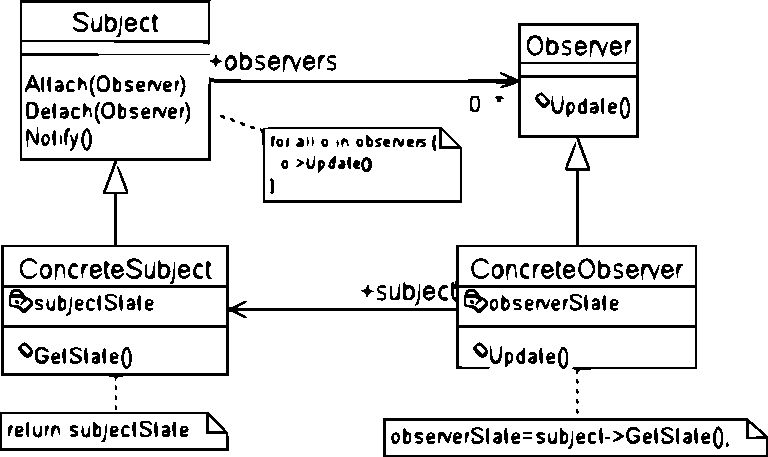
\includegraphics[scale=0.80]{immagini/observer.pdf}
 \caption{Pattern Observer}
 \label{fig:observer}
\end{figure}

Nella panoramica sui risvolti più interessanti del codice è necessario citare il modello \textbf{signal-slot} offerto dalle librerie Qt, sebbene questo non sia stato propriamente applicato quanto piacevolmente adottato per migliorare il software e rendere più flessibile la programmazione. In parole povere, questo modello si propone come un'ottima alternativa al sistema delle callback, mimando il pattern \textit{Observer} (si veda figura \ref{fig:observer}) e al contempo liberando l'utente dalla scrittura del codice di controllo ridondante e sempre uguale che vi fa da contorno.

Gli attori sono banalmente presentati e descritti come:
\begin{description}
 \item[signal] Sono emessi da un oggetto quando muta il proprio stato interno in un modo che può essere interessante per chi lo possiede o per chi lo osserva. Intuitivamente solo chi definisce il segnale e le sottoclassi possono emettere la notifica di cambiamento. Quando un segnale viene emesso, tutti gli slot ad esso collegati vengono invocati in successione, indipendentemente dal ciclo di esecuzione principale (ad esempio, in caso di interfacce grafiche).
 \item[slot] Uno slot rappresenta un metodo avente firma identica in tutto e per tutto ai segnali al quale lo si vuole collegare, che viene invocato quando tali segnali sono emessi. In quanto funzione, esso può essere chiamato anche direttamente da altre classi, se pubblico, o da classi ereditarie.
\end{description}

Alcune particolarità che distinguono la coppia \textit{signal-slot} dagli altri metodi sono:
\begin{itemize}
 \item L'essere un metodo type-safe: le firme di signal e slot devono coincidere e non vi è la possibilità di confusione o errori sul passaggio di valori.
 \item La capacità di abbattere l'accoppiamento fra le classi, riducendolo al minimo indispensabile per permettere la comunicazione fra esse. Di fatto chi emette un segnale non si preoccupa minimamente di chi siano i riceventi.
 \item Arbitrarietà sul numero e sul tipo di componenti passate come argomento alla chiamata.
 \item Possibilità di connettere più segnali ad un unico slot, più slot ad un unico segnale e perfino più segnali in cascata fra loro.
\end{itemize}
Tutto sommato, insomma, il meccanismo in questione rappresenta una utile e potente tecnica di programmazione capace di semplificare non poco le cose.

Ovviamente la questione è sufficientemente più articolata e complessa; si possono per esempio definire slot virtuali e realizzare cose ben più raffinate. Ad ogni modo non è questa la sede per discutere di un metodo dovuto e legato ad una libreria semplicemente sfruttata durante lo sviluppo di QSapecNG, poiché la documentazione che accompagna tale libreria risulta essere più che esaustiva in merito.

\section{Design Patterns}
A conclusione di questa panoramica sulle tecniche di sviluppo adottate, vengono descritti alcuni degli approcci utilizzati per risolvere problemi tipici della programmazione ad oggetti, riscontrabili anche nel software in esame. Queste tecniche prendono il nome di \textit{Design Pattern} (schema di progettazione) e rappresentano soluzioni generali a problemi ricorrenti nella programmazione. I design pattern non sono oggetti o librerie pronte all'uso quanto piuttosto modelli da applicare in frangenti noti, riuscendo a risolvere così in modo elegante, pulito e maggiormente manutenibile le problematiche reali.

\paragraph{Pattern Monostate}

\begin{lstlisting}[basicstyle=\small,language=C++,caption={Pattern Singleton},float,label={lst:singleton},captionpos=b,frame=lines]
 class Singleton
 {
 private:
   static Singleton* instance;

   Singleton(): some_data(0) { }
   ~Singleton() { }
   Singleton(const Singleton &);
   Singleton & operator=(const Singleton &);

   int some_data;

 public:
   static Singleton& get_instance();

   void increment() { ++some_data; }
   int get_data() { return some_data; }
 };


 Singleton Singleton::instance = 0;


 Singleton& Singleton::get_instance()
 {
   if(!instance)
     instance = new Singleton;

   return *instance;
 }
\end{lstlisting}

\begin{lstlisting}[basicstyle=\small,language=C++,caption={Pattern Monostate},float,label={lst:monostate},captionpos=b,frame=lines]
 class Monostate
 {
 private:
   static int some_data;

 public:
   Monostate() { }
   ~Monostate() { } 

   void increment() { ++Monostate::some_data; }
   int get_data() { return Monostate::some_data; }
 };


 int Monostate::some_data = 0;
\end{lstlisting}

\begin{lstlisting}[basicstyle=\small,language=C++,caption={Pattern Monostate in QSapecNG},float,label={lst:qmono},captionpos=b,frame=lines]
class SettingsManager;


class Settings
{

friend class SettingsManager;

public:
  Settings() { }

  inline int logLvl() const
    { return logLvl_; }

  inline QColor debugColor() const
    { return debugColor_; }

  inline QColor infoColor() const
    { return infoColor_; }

  // ...

private:
  static int logLvl_;
  static QColor debugColor_;
  static QColor infoColor_;

  // ...

};

int Settings::logLvl_ = 0;
QColor Settings::debugColor_ = QColor(Qt::black);
QColor Settings::infoColor_ = QColor(Qt::black);

// ...


class SettingsManager
{

public:
  inline void setLogLvl(int lvl)
    { Settings::logLvl_= lvl; }

  inline void setDebugColor(const QColor& color)
    { Settings::debugColor_ = color; }

  inline void setInfoColor(const QColor& color)
    { Settings::infoColor_ = color; }

  // ...

};
\end{lstlisting}

Uno dei pattern più discussi e criticati è il \textit{Singleton} (listato \ref{lst:singleton}), un approccio atto a rendere centralizzata in un singolo oggetto la possibilità di istanziare una classe e disporne riferimenti per l'accesso ai dati. Risulta utile quando è necessario che sia un solo oggetto a gestire l'accesso a determinate funzioni e parametri all'interno dell'intero ambiente. Il rovescio della medaglia è dato dal fatto che l'uso di questo pattern rende difficoltose le fasi di testing del software ed introduce uno stato globale nell'applicazione. Riduce inoltre le potenzialità del parallelismo, obbligando la serializzazione in accesso e qualcuno lo annota addirittura fra gli \textit{anti-pattern}, ovvero tutte quelle tecniche che rappresentano un modo sbagliato di procedere nella programmazione.\\
Il problema fondamentale del pattern Singleton è che esso rende unico l'oggetto istanziabile e utilizzabile per l'accesso ai dati, rappresentando una sorta di collo di bottiglia per l'uso di informazioni che sarebbero altrimenti rese a livello globale. Se si permettesse, infatti, la creazione di più oggetti Singleton, ognuno di essi conterrebbe informazioni che finirebbero con l'essere discordanti nel tempo, rendendo di fatto incoerente lo stato globale all'interno del sistema. In altri termini, istanziando più oggetti Singleton, ogni loro utilizzatore avrebbe un'immagine diversa del sistema, in base all'oggetto a cui accede.

Come alternativa al pattern Singleton, è stato proposto negli anni il pattern \textit{Monostate}\graffito{Il pattern Monostate espone gli stessi punti deboli del pattern Singleton ma è maggiormente apprezzato perché favorisce soluzioni più pulite ai problemi intrinseci} (listato \ref{lst:monostate}). Questo è definito a livello concettuale come un Singleton ma sfrutta la possibilità di rovesciare il punto di vista. Non è più l'oggetto che gestisce i dati ad essere unico nel sistema, bensì sono i dati ad essere unici, ovvero statici e privati. Questo non risolve, in realtà, tutte le problematiche legate al pattern Singleton, sebbene ne renda più snello e chiaro l'uso. Un oggetto Monostate si presta meglio anche all'uso in ambienti paralleli, poiché la serializzazione non avviene più all'esterno ma può essere spostata all'interno dell'oggetto. Inoltre viene meno la necessità di avere un unico oggetto istanziato all'interno del sistema e se ne possono avere in numero illimitato.

All'interno di QSapecNG il pattern Monostate è stato utilizzato principalmente per centralizzare la gestione dei dati di configurazione dell'interfaccia grafica, così da permetterne un facile accesso da qualsiasi punto. Il modello adottato è leggermente diverso da quello visto nel listato \ref{lst:monostate} ed è parzialmente riportato nel listato \ref{lst:qmono}, dove si nota come siano suddivise fra loro la classe utilizzata per l'accesso in lettura e la memorizzazione dei dati e quella indicata per l'accesso in scrittura.

\paragraph{Pattern Builder}

\begin{figure}[ht]
 \centering
 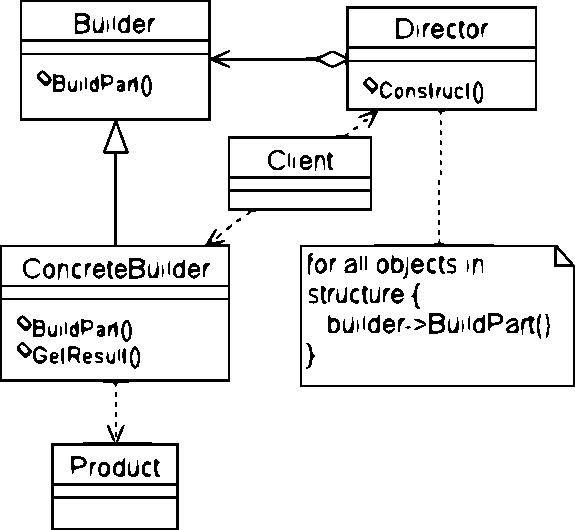
\includegraphics[scale=0.80]{immagini/builder.pdf}
 \caption{Pattern Builder}
 \label{fig:builder}
\end{figure}

Il pattern \textit{Builder} (riportato in figura \ref{fig:builder}) si è rivelato il più flessibile e meglio integrato nell'intera struttura del software QSapecNG. Gli intenti alla base di questo modello sono i seguenti:
\begin{itemize}
 \item Separare le procedure di costruzione di un oggetto complesso dalla sua rappresentazione.
 \item Fare in modo che uno stesso processo di generazione possa dar luogo a più rappresentazioni diverse.
\end{itemize}
Questo lo si ottiene a partire da due classi, chiamate spesso in letteratura \textit{Director} e \textit{Builder}, di cui la seconda è una semplice interfaccia. Le rappresentazioni concrete di Builder andranno quindi a costituire il processo di generazione dei diversi oggetti, mentre a Director sarà demandato il compito di orchestrare correttamente la chiamata dei singoli metodi. Infine, le classi che ereditano da Builder potranno fornire metodi ausiliari per recuperare quanto creato al loro interno.

\begin{lstlisting}[basicstyle=\small,language=C++,caption={Builder in QSapecNG},float,label={lst:builder},captionpos=b,frame=lines]
class abstract_builder
{

public:
  enum const_vertex { GROUND = 0 };

  enum dual_component_type
    { R, G, L, C, V, I, VM, AM };

  enum quad_component_type
    { VCCS, VCVS, CCCS, CCVS, AO, n, K };

public:
  virtual ~abstract_builder() { }

  virtual void add_circuit_properties(
    std::map<std::string, std::string> map) = 0;
  virtual void add_circuit_property(
    std::string name, std::string value) = 0;

  virtual void add_wire_component(
      std::map<std::string, std::string> props =
        std::map<std::string, std::string>()
    ) = 0;

  virtual void add_out_component(
      unsigned int v,
      std::map<std::string, std::string> props =
        std::map<std::string, std::string>()
    ) = 0;

  virtual void add_dual_component(
      dual_component_type c_type,
      std::string name, double value, bool symbolic,
      unsigned int va, unsigned int vb,
      std::map<std::string, std::string> props =
        std::map<std::string, std::string>()
    ) = 0;

  virtual void add_quad_component(
      quad_component_type c_type,
      std::string name, double value, bool symbolic,
      unsigned int va, unsigned int vb,
      unsigned int vac, unsigned int vbc,
      std::map<std::string, std::string> props =
        std::map<std::string, std::string>()
    ) = 0;

  virtual void add_unknow_component(
      std::map<std::string, std::string> props =
        std::map<std::string, std::string>()
    ) = 0;

  virtual void flush() = 0;

};
\end{lstlisting}

\begin{lstlisting}[basicstyle=\small,language=C++,caption={Director in QSapecNG},float,label={lst:parser},captionpos=b,frame=lines]
class abstract_parser
{

public:
  abstract_parser() { }
  virtual ~abstract_parser() { }

  virtual void parse(abstract_builder& builder) = 0;

};
\end{lstlisting}

Astraendo ulteriormente si può pensare di rendere anche la classe Director una semplice interfaccia, costruendo un doppio albero di ereditarietà che permetta la costruzione di oggetti diversi a partire da sorgenti diverse. Questo è stato l'approccio utilizzato in QSapecNG e le interfacce base sono riportate integralmente nei listati \ref{lst:builder} e \ref{lst:parser}.

Le potenzialità di questo approccio sono state sfruttate in diversi punti del software. I più rilevanti sono:
\begin{itemize}
 \item Una classe ereditata da Builder capace di costruire circuiti schematici in base alle sollecitazioni.
 \item Una classe ereditata da Parser capace di leggere ed interpretare circuiti schematici.
 \item Una classe ereditata da Builder per la generazione del circuito come coppia di grafi in corrente e in tensione.
 \item Più classi ideate con lo scopo di leggere e scrivere file su disco, per la memorizzazione ed il caricamento di dati.
\end{itemize}
Questi sono solamente alcuni dei casi in cui è stato applicato il pattern in questione ma se ne intuisce facilmente l'utilità.\\
Immaginiamo per esempio di voler generare, a partire da un disegno schematico, una coppia di grafi in corrente e in tensione: basterà agganciare l'apposito Builder al Director in grado di leggere lo schema. Non solo, volendo si può anche by-passare il disegno dello schema e perfino l'avvio dell'interfaccia grafica, utilizzando un Parser per la lettura di file da disco unito al Builder di cui sopra. Se poi il disegno dello schema lo si vuole evitare perché, semplicemente, lo si è già disegnato, all'ultimo Parser utilizzato basterà legare un Builder capace di generare il circuito schematico ed il gioco è fatto.\\
Questa tecnica può anche essere utilizzata in frangenti meno ovvi, ad esempio nelle fasi di copia-incolla, leggendo da uno schema circuitale su di uno flusso di testo e quindi, attingendo da quest'ultimo, sfruttando un costruttore per incollare quanto copiato.

Riassumendo quindi si nota come il pattern Builder si presti a realizzare una gran quantità di interconnessioni fra oggetti anche in aree diverse del software, disaccoppiando o rendendo comunque minimo l'accoppiamento fra essi e permettendo di risolvere elegantemente problemi che avrebbero altrimenti richiesto la stesura di classi dalla collocazione dubbia, ambigue nel comportamento e difficilmente manutenibili.

\paragraph{Pattern Template Method}

\begin{figure}[ht]
 \centering
 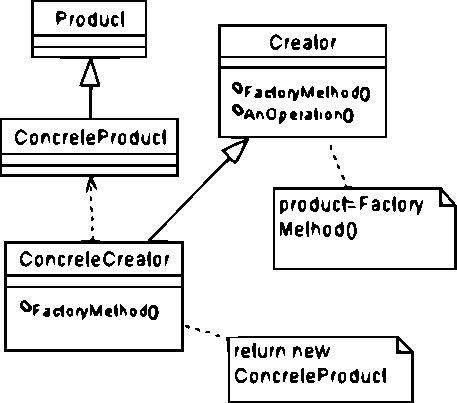
\includegraphics{immagini/factorymethod.pdf}
 \caption{Pattern Factory Method}
 \label{fig:factorymethod}
\end{figure}

\begin{lstlisting}[basicstyle=\small,language=C++,caption={Pattern Template Method in QSapecNG},float,label={lst:templatemethod},captionpos=b,frame=lines]
struct functor
{

public:
  std::pair< std::vector<double>, std::vector<double> >
  operator()
    (
      const metacircuit::expression& numerator,
      const metacircuit::expression& denominator,
      std::map< std::string, double > values
    )
  {
    std::map< int, double > real_num = synthesis(numerator, values);
    std::map< int, double > real_den = synthesis(denominator, values);
    return op(real_num, real_den);
  }

protected:
  virtual std::pair< std::vector<double>, std::vector<double> >
    op(std::map< int, double > num, std::map< int, double > den) = 0;

private:
  std::map< int, double >
  synthesis(
      const metacircuit::expression& expr,
      std::map< std::string, double > values
    )
  {
    // ...
  }

};
\end{lstlisting}

Questo pattern (illustrato in figura \ref{fig:factorymethod}) è particolarmente interessante poiché sfrutta i principi della \textit{IoC} (\textit{Inversion of Control}, o inversione di controllo), ovvero ribalta il meccanismo dell'ereditarietà. Non sono più infatti le classi che ereditano a chiamare i metodi della classe base, bensì sarà quest'ultima ad invocare uno o più metodi lasciati da implementare alle classi derivate. Si riesce così a definire la struttura di un algoritmo delegando alle sottoclassi il compito di implementare i passi chiave, permettendone una personalizzazione ma evitando al contempo la duplicazione di codice. Questo modus operandi (largamente usato anche in diversi framework noti) è detto \textit{Principio di Hollywood: ``non chiamarci, ti chiameremo noi''}.

All'interno del codice di QSapecNG questo modello è stato adottato per le diverse funzioni applicabili ad un determinato circuito, in modo da costruire un'architettura robusta ma personalizzabile per l'analisi dei dati derivati dalla simulazione. Nel listato \ref{lst:templatemethod} è riportata la classe base (classe funzione, per inciso), dove si nota la chiamata del metodo la cui implementazione è lasciata come onere alle classi derivate.

Per completezza di informazione bisogna dire che da questa classe base ereditano classi come ad esempio \textit{gain} o \textit{zeros} e così via, il cui nome è esplicativo della funzione svolta. Salendo di livello e spostandoci da SapecNG, dove tale modello è sviluppato, a QSapecNG, dove tale modello è effettivamente sfruttato, si può osservare come queste classi derivate si vadano a collocare in un'architettura di \textit{traits} che ne completa l'informazione associata, arricchendola nell'ottica dell'uso all'interno dell'interfaccia grafica. Questo lascia intuire come le varie parti del sistema e i diversi pattern possano venire in contatto e collaborare fra loro per uno scopo comune.

\chapter{Note di Programmazione}

Il software sviluppato ha sposato alcuni dei principi base della programmazione ad oggetti e non, presentandosi di conseguenza con un codice ricco di caratteristiche interessanti. Alcuni degli aspetti più rilevanti, una breve infarinatura su cosa sia proposto concretamente, sono discussi in questo capitolo, nel tentativo di non appesantire la discussione con complessi dettagli tecnici e al contempo cercando di offrire una visione d'insieme su quelli che appaiono come gli spunti più interessanti.

\section{Separazione backend/frontend}

\begin{figure}
 \centering
 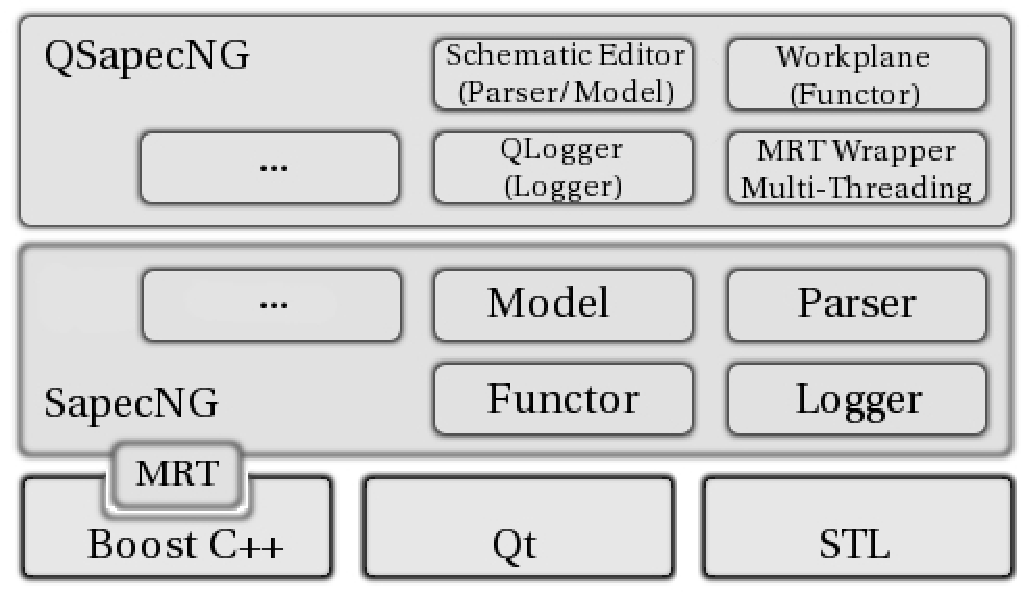
\includegraphics[scale=0.6]{immagini/qsapecngschema.pdf}
 \caption{QSapecNG (schema)}
 \label{fig:qsapecngschema}
\end{figure}

QSapecNG adotta un modello stratificato illustrato (in maniera imperfetta) in figura \ref{fig:qsapecngschema}.\graffito{Nulla vieta di sviluppare un adattamento che sfrutti SapecNG e presenti una interfaccia basata sulle librerie Gtk} Imperfetta o per meglio dire incompleta poiché il riquadro \textit{Qt} andrebbe sostituito in realtà con la dicitura: qualsiasi libreria grafica disponibile.

L'immagine è infatti fedelmente legata a QSapecNG stesso ma lo sviluppo del software si è incentrato su un'ottica di separazione totale fra \textit{backend} e \textit{frontend}, ovvero fra SapecNG e QSapecNG. Questo ha permesso, nel complesso, di sviluppare una sorta di framework per la risoluzione simbolica e costruire quindi su di esso un'interfaccia grafica che, presentando un ambiente di disegno e gli strumenti necessari all'analisi, si limitasse a usufruire di quanto offerto dal livello sottostante.

Rifacendosi quindi al caso specifico, si capisce perché il software sia stato rappresentato come in figura \ref{fig:qsapecngschema}, dove per aiutare la comprensione sono stati indicati alcuni dei moduli presenti ai diversi livelli, sottolineando come questi siano fra di loro legati, ovvero come in alcuni casi basino il proprio funzionamento su altri moduli specifici.

Il cuore principale, l'ambiente che ospita gli algoritmi di risoluzione simbolica, le strutture dati utili allo scopo, gli strumenti di analisi utilizzabili per rielaborare i valori ottenuti, è rappresentato da SapecNG, codice costruito prevalentemente con l'ausilio di Boost C++ e della libreria standard STL. Nel caso in esame è stato illustrato anche, graficamente, come il framework realizzato abbia contribuito con un apporto di nuovi algoritmi alla libreria BGL.

Su di esso, a sua volta e non solo, se si considera il mattone rappresentato dalla libreria grafica utilizzata, poggia l'ambiente finale offerto all'utente, il quale non reinventa la ruota e, in linea teorica, dovrebbe tendere a non espandere le funzionalità del software in questa sede, bensì facendole migrare di livello verso il basso.

Questo permette una netta separazione fra backend e frontend e quindi lo sviluppo, nonostante l'estrema portabilità del codice già presente, di ulteriori e molteplici ambienti basati sul framework proposto nella forma di SapecNG.

\section{SUPER: Scalabile, Usabile, Portabile, Evolvibile, Riusabile}

Il codice sviluppato presenta svariate caratteristiche interessanti, quali quelle solitamente discusse analizzando gli aspetti di qualità del software. In realtà sono ben più di quante sopra elencate, acronimo delle quali si propone di rispecchiare il complesso della loro somma, e di seguito saranno brevemente introdotte e spiegate alcune delle principali, senza la pretesa di essere esaustivi nel numero.

Alcuni dei punti cardine si possono riassumere in:
\begin{description}
 \item[Efficienza e Prestazioni] Un'attenzione particolare è stata posta nello sfruttamento delle risorse, sia in termini di memoria che di CPU; laddove risultasse poi impossibile abbattere i tempi di computazione (ad esempio nei processi di ricerca degli alberi di copertura comuni fra due grafi, il cui algoritmo ha elevata complessità) sono stati adottati modelli multi-threading per rendere fruibile l'ambiente anche durante pesanti fasi di calcolo.
 \item[Usabilità] L'interfaccia grafica e il modello di utilizzo del software sono stati concepiti in un'ottica di massima flessibilità, personalizzazione e semplicità d'uso, così da venire incontro all'utente presentandosi fin da subito come un ambiente intuitivo, ben amalgamato nelle sue molteplici parti e facile da usare tanto per gli esperti del settore quanto per i neofiti.
 \item[Scalabilità] L'introduzione del multi-threading nelle fasi risolutive ha permesso di andare incontro a richieste sia semplici che esose, senza penalizzazioni in alcun caso e sposando perfettamente le differenze di complessità che possono esserci nelle richieste dei diversi utenti; il modello adottato difficilmente richiederà correzioni atte ad accettare determinati circuiti, poiché nei limiti delle risorse di calcolo esso è in grado di soddisfare tutte le richieste, sebbene possa godere effettivamente di un incremento proprio in termini di risorse di calcolo migliorando le proprie prestazioni.
 \item[Manutenibilità e Riparabilità] L'applicazione dei più diffusi e flessibili pattern di sviluppo, affiancati ai modelli proposti dalle stesse librerie coinvolte, rende la manutenzione e la correzione di eventuali errori un processo semplice ed intuitivo per chi abbia padronanza degli strumenti coinvolti.
 \item[Evolvibilità] Fin da subito è stato messo un accento sulla possibilità di evoluzioni future del software, da cui un'attenta e oculata fase di design e progettazione che lasciasse ampio respiro a modifiche e aggiunte apportate in un secondo momento, senza dover ricorrere necessariamente a stravolgimenti del codice.
 \item[Riusabilità] Quanto già esposto parla da solo: un framework di base per lo sviluppo senza limiti di ambienti di disegno e algoritmi proposti per l'integrazione in librerie di software generico urlano a voce alta la tendenza del codice all'estrema riusabilità.
 \item[Portabilità] L'uso delle librerie Qt, portabili per definizione, Boost C++ e l'attenzione posta nel non legarsi a specifiche interrogazioni dipendenti dal sistema in uso, hanno reso QSapecNG ad oggi funzionante su un'ampia gamma di sistemi, sfociando dalla sua concezione iniziale di un ambiente per il disegno elettronico e l'analisi simbolica su sistemi unix-like in un programma multi-piattaforma.
\end{description}

Tutto questo e molto altro ancora fanno si che SapecNG e QSapecNG si propongano come modelli estremamente flessibili per dedicare loro attenzioni in merito a sviluppi futuri.



\cleardoublepage
\part{Conclusioni}

\thispagestyle{empty}
\null\vspace{\stretch{1}}
\begin{flushright}
\setlength{\epigraphwidth}{21em}
\epigraph{
\footnotesize{Ha due importanti vantaggi $[[$\ldots$]]$. Uno, costa un po' meno; due, ha stampate in copertina, a grandi caratteri che ispirano fiducia, le parole \textsc{non fatevi prendere dal panico}.}
}{\footnotesize{Guida galattica per autostoppisti\\ Douglas Adams}}
\end{flushright}\vspace{\stretch{2}}\null

\chapter{Conclusioni}

Gli studi riguardanti l'analisi simbolica nascono e si sviluppano inizialmente in ambito accademico, dove trovano terreno fertile per quanto riguarda anche la loro applicazione. Le teorie ad essi collegate attraversano lo spazio dell'analisi matriciale, relegando la loro effettiva applicabilità a piccoli problemi modello, per sfociare col tempo nello spazio dei grafi da cui, sposandosi con la crescente potenza computazionale delle macchine che li eseguono, nascono algoritmi performanti e in grado di attirare l'attenzione di studiosi e non solo. L'ovvia conseguenza consiste nell'interesse del mondo industriale che vede nell'analisi simbolica uno strumento da accostare a quelli già esistenti per scopi specifici, ottenendo così una visione d'insieme più chiara per quanto riguarda i propri progetti.

Questo strumento è quindi soggetto ad un interesse interdisciplinare in ambito teorico (per esempio, ha attinto dal campo dell'elettronica e dell'informatica), oltre ad essere oggetto di un interesse trasversale fra diversi ambiti apparentemente distanti fra loro, come quello del mondo accademico e quello del modello industriale.

L'uso che tanto gli studenti delle scuole medie superiori quanto gli universitari ne possono fare, così come il vantaggio che uno sviluppatore hardware può trarne, è indubbio. La sola limitazione è data dal ridotto parco di elementi effettivamente sfruttabile a tale scopo, il che può rappresentare un freno alle possibilità di utilizzo. Ciò nonostante, basti pensare che i primi studi si erano concentrati sui soli componenti di tipo ammettenza, per poi estendere l'analisi agli elementi di tipo impedenza e quindi trovare soluzioni e modelli alternativi per generatori, generatori controllati, amplificatore operazionale e così via. L'obiettivo è quindi, col tempo, quello di estendere sempre più il fronte della circuiteria analizzabile in modo simbolico, rendendo questa pratica maggiormente fruibile in tutti i settori su cui si affaccia.

\section{Sviluppi futuri}
Per quanto riguarda il software sviluppato, esso mette in campo tutto il necessario per svolgere le procedure di analisi simbolica, separando nettamente la parte operativa dall'interfaccia utente, così che se ne possa usufruire anche in altro modo (ad esempio, sviluppando interfacce specifiche per altri ambienti o sistemi).

\paragraph{}
Sulla base della struttura già presente, pensata fin da principio per essere estesa e adatta allo scopo a tutti i livelli, uno dei primi passi necessari sarà quello di ampliare il parco procedure per l'analisi delle funzioni di trasferimento. In quest'ottica, potrebbe essere interessante abbracciare l'ipotesi di un'analisi parametrica, così da poter ospitare in un unico grafico più curve relative ad un determinato circuito, offrendo la possibilità di un confronto e un'analisi maggiormente specifica.

Un altro concetto interessante da approfondire è quello dei sottocircuiti, uno strumento che permette di lasciare all'utente la libertà di sviluppare propri componenti personalizzati da inserire in circuiti più ampi e da riutilizzare nel tempo. Molti simulatori di diverso genere, già presenti nel panorama informatico, propongono questa opzione, che non ha esistato a mostrarsi in tutta la sua versatilità. Questa innovazione potrebbe ripercuotersi anche nella stesura di un pacchetto di componenti distribuito col software, per permettere all'utente finale di attingere ad un gruppo di elementi già sviluppati.

Sfociando nella parte più teorica che sta dietro al software, una delle evoluzioni più importanti sarebbe quella della traduzione di quei componenti, ad oggi non trattabili, nella forma di coppia di grafi in tensione e in corrente. Questo permetterebbe un'immediata inclusione di essi all'interno dell'ambiente di disegno e quindi una immediata fruibilità, poiché per come è stato concepito l'intero software è già predisposto per accogliere facilmente nuovi elementi in futuro.

\paragraph{}
Con questa breve carrellata di alcuni degli spunti più interessanti che potrebbero muovere lo sviluppo futuro di QSapecNG, è necessario sottolineare che autore e relatori del lavoro di tesi hanno deciso di mettere a disposizione della comunità il codice sviluppato, così che questo possa essere studiato e ad esso possano essere apportati miglioramenti di ogni genere. La direzione presa rappresenta un'opportunità di crescita per QSapecNG, offrendo la possibilità di farsi conoscere nell'ambiente e di venire incontro alle necessità del singolo con l'apporto di tutti.


\section{Il software QSapecNG}
QSapecNG è rilasciato sotto licenza GPLv3 e, insieme al codice, verrà presto reso disponibile al pubblico nella sua prima release stabile. Essendo il progetto nato in seno all'Università di Firenze, verranno sfruttati in linea di massima i canali di quest'ultima per rendere disponibile quanto realizzato; l'indirizzo di riferimento (lo stesso che ha presentato al pubblico SapWin e SapecNG) sarà:\\
\url{http://www.cirlab.unifi.it/}



\appendix

\cleardoublepage
\part{Appendici}
\chapter{Generazione schema da netlist}

Durante lo sviluppo di sistemi CAD per il disegno di circuiti elettrici, la compatibilità con formati di ingresso presenti sul panorama attuale rappresenta un fattore di flessibilità molto importante. Può risultare utile la lettura di file generati da software simili ma aventi caratteristiche diverse, come ad esempio risolutori numerici e simbolici o anche solo risolutori di generazioni successive. Non tutti i formati, però, recano con sé informazioni riguardanti la dislocazione grafica dei componenti all'interno di uno spazio di disegno, addirittura spesso il problema è dato dal fatto che dati riguardanti la struttura del circuito e la sua rappresentazione grafica sono suddivisi in file diversi.

Basti pensare ad esempio alle \textit{netlist} prodotte come formato intermedio da SapWin \cite{sapwin}, di cui un esempio è riportato nel listato \ref{netlist} dove è descritto il modello relativo ad un amplificatore operazionale. Di fatto le informazioni presenti indicano i nodi ai quali il componente si aggancia, il suo valore numerico e il suo stato (se deve essere cioè trattato effettivamente come valore numerico o come componente simbolico). Niente di tutto ciò, intuitivamente, può aiutare nella generazione di uno schema.\\
Una ricostruzione intelligente, coerente e mirata a ridurre lo spazio di occupazione è pertanto uno dei nodi cruciali per la gestioni di modelli di questo genere. L'idea alla base del lavoro riportato in questa appendice è che grazie ai pochi dati ricavabili da una netlist e alle informazioni aprioristiche sulla struttura grafica dei componenti, si possa trovare una dislocazione ottima in grado di minimizzare lo spazio occupato e ridurre alcuni altri fattori di interesse che verranno illustrati in seguito.
\lstset{basicstyle=\small, language=, breaklines, breakatwhitespace}

\begin{lstlisting}[caption={Esempio di netlist},float,captionpos=b,label=netlist,frame=lines]
Vin 0 1 1 1
Rs 2 1 1 1
Rin 0 2 1 1
E 0 3 0 2 1 1
Rout 4 3 1 1
Rl 0 4 1 1
.OUT 4
.END
\end{lstlisting}

\paragraph{L'ambiente di disegno}
Collocando questo studio all'interno del software di disegno QSapecNG, risulta utile alla comprensione introdurre alcune nozioni su come tale ambiente si presenti e su quali siano i vincoli a cui bisogna sottostare.

Innanzitutto si noti che l'area sfruttabile è pressochè illimitata, il che vuol dire che non si hanno vincoli sulla superficie occupabile. Di contro, lo scopo è quello di minimizzarla così da rendere più compatta la rappresentazione. La scelta ricadrà su un modello piuttosto ovvio, ovvero sulla minimizzazione del perimetro di occupazione. Osservando che l'area di disegno è suddivisa in celle attraverso una griglia, si può pensare quindi di esprimere altezza e larghezza dello spazio occupato in termini di numero di celle (o meglio, in numero di divisori, punti sulla griglia, tali per cui $ N $ divisori indicano un'occupazione di $ N-1 $ celle) e sfruttare questa notazione all'interno dell'intero modello. Come vedremo, questa tecnica semplificherà molto le cose, permettendo ad esempio di definire anche un certo discostamento fra i diversi componenti sempre come numero di celle della griglia.

Per quanto riguarda i componenti, in questo frangente si può pensare di sfruttarne una conoscenza aprioristica sulla loro forma, derivante dal software stesso. In altri termini, si possono descrivere anche per essi altezza e larghezza come numero di celle occupate. Questo aiuta a rendere conforme la descrizione delle dimensioni dell'area utilizzata con quelle dei componenti; così facendo si possono pertanto facilmente definire vincoli che mettano in relazione tali aspetti.

\begin{figure}[ht]
 \centering
 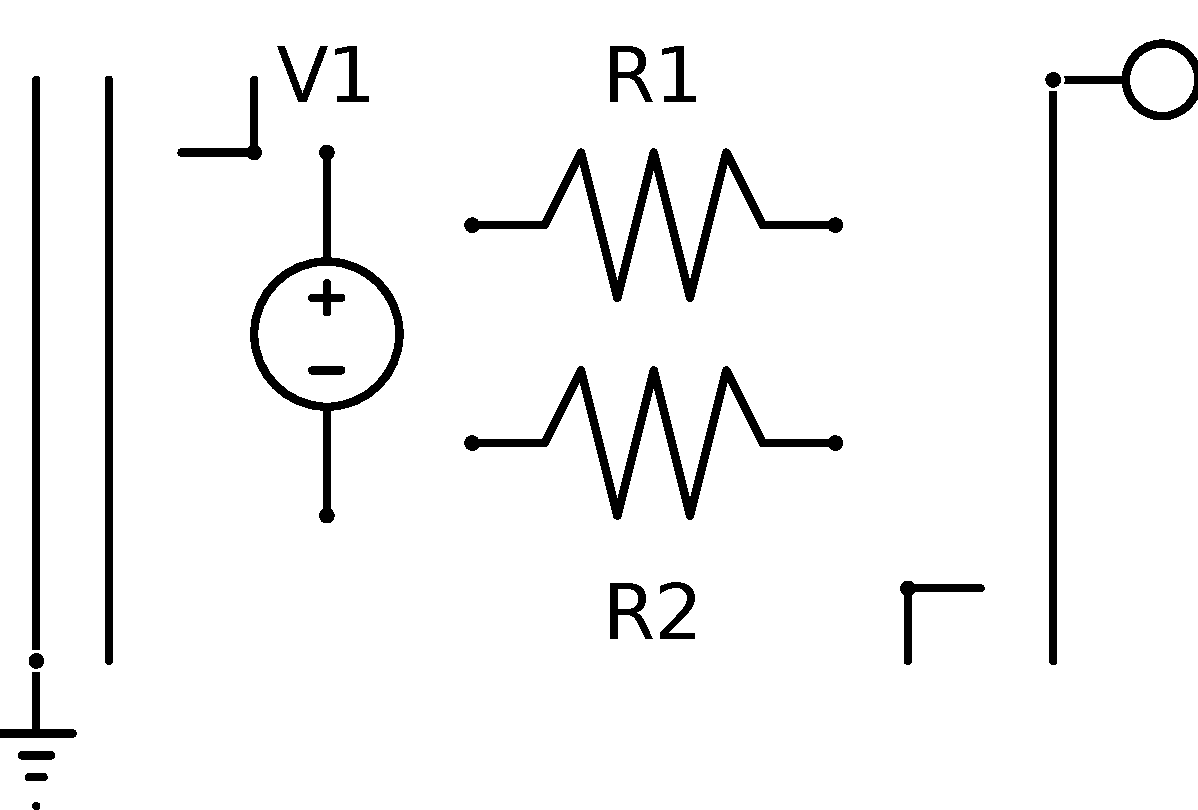
\includegraphics[scale=0.35]{immagini/design.pdf}
 \caption{Esempio di design per la ricostruzione}
 \label{cdes}
\end{figure}

La ricostruzione del circuito all'interno dell'ambiente di disegno avverrà sfruttando le diverse tipologie di fili disponibili, ovvero utilizzando ponticelli per la stesura dei collegamenti a partire dai componenti. Tali fili saranno diretti a punti di aggancio immediatamente esterni all'area occupata, dislocati sulla sinistra e sulla destra di essa, in numero bilanciato. Un'immagine che esemplifica quanto detto è riportata in figura \ref{cdes} dove, in particolare, è stato anche segnato il limite superiore-sinistro e inferiore-destro dello spazio occupato Il circuito è la ricostruzione di un divisore di tensione e i tre fili di riferimento possono essere assimilati a massa, tensione di uscita e punto di snodo fra il generatore e una delle due resistenze.

\paragraph{Il modello}
La descrizione del modello è svolta per passi, introducendo via via parametri e variabili e spiegandone il loro scopo e la loro utilità. Per una rappresentazione globale del modello utilizzato si faccia riferimento al listato \ref{allmod}. Si tenga presente che, per astrarre dal caso specifico, si sono separati il modello stesso dai dati, ottenendo così una rappresentazione generica del problema adattabile a qualsiasi situazione.

Il primo passo consiste nella definizione di un insieme che contenga i nostri componenti, identificabili per nome (così da facilitare le cose). Letteralmente:
\small
\begin{verbatim}
 set ITEM ;
\end{verbatim}
\normalsize
Il file dati potrebbe riportare molto semplicemente, ad esempio, nel caso del divisore di tensione in figura \ref{cdes}:
\small
\begin{verbatim}
 set ITEM := V1 R1 R2 ;
\end{verbatim}
\normalsize

A supporto dell'insieme dei componenti vi sono alcuni parametri su di esso definiti, per ogni elemento, ovvero larghezza e altezza dell'oggetto, oltre che il numero di nodi che devono tendere ad avvicinarsi al lato sinistro dello spazio occupato e il numero di nodi che viceversa devono tendere dal lato opposto (questo sarà strettamente dipendente dalla dislocazione dei punti di aggancio subito adiacenti all'area occupata). Infine, vi sarà un parametro che indicherà lo scostamento desiderato fra due componenti diversi, così da poter imporre una divisione a priori interna allo schema. Otteniamo:
\small
\begin{verbatim}
 param Width {i in ITEM} ;
 param Height {i in ITEM} ;
 param NL {i in ITEM} ;
 param NR {i in ITEM} ;
 param delta ;
\end{verbatim}
\normalsize
Sempre rifacendosi all'esempio del divisore di tensione, potremmo avere:
\small
\begin{verbatim}
 param Width :=
    V1 3
    R1 6
    R2 6
  ;

 param Height :=
    V1 6
    R1 3
    R2 3
  ;

 param NL :=
    V1 2
    R1 1
    R2 1
  ;

 param NR :=
    V1 0
    R1 1
    R2 1
  ;

 param delta := 1 ;
\end{verbatim}
\normalsize
Legando questi dati all'ambiente di disegno, si possono ricostruire nella direzione opposta alcune caratteristiche significative dei componenti.\\
Ad esempio, per quanto riguarda il generatore di tensione, si osserva che esso è rappresentato in posizione verticale ed ha un'occupazione di due celle in larghezza e cinque celle in altezza (ovvero tre separatori in larghezza racchiudono, evidentemente, due celle e in modo simile vale anche per l'altezza), mentre le resistenze sono disposte in posizione orizzontale, facilmente deducibile dai dati riguardanti l'area occupata.\\
In merito alle richieste sui nodi, le quali influiranno in seguito sul processo di dislocazione, si nota che il generatore di tensione ha una tendenza maggiore a spostarsi verso il lato sinistro dello spazio occupato (infatti, supponendo di avere tre nodi all'interno del circuito, il nodo massa e il primo snodo fra generatore e resistenza saranno posizionati sul lato sinistro dell'area occupata, pertanto necessariamente viene richiesta in questo caso una vicinanza a tale lato); in maniera simile le due resistenze sono entrambe connesse al terzo dei tre nodi presenti (posto a destra dello spazio occupato) e ad uno dei due nodi citati in precedenza, pertanto dividono le loro richieste fra i due lati dell'area occupata, mostrando una tendenza ad occupare posizioni centrali.\\
Si faccia riferimento alla figura \ref{vdiv_schema} per aiutare la comprensione dei dati.\\
L'ultimo parametro, \textit{delta}, indica banalmente un valore di discostamento che si desidera avere fra due componenti affiancati orizzontalmente o verticalmente. Vedremo come, in seguito, sarà utilizzato a tale scopo.

\begin{figure}[ht]
 \centering
 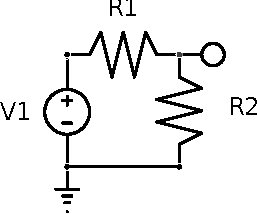
\includegraphics[scale=1]{immagini/vdiv_schema.pdf}
 \caption{Divisore di tensione}
 \label{vdiv_schema}
\end{figure}

Prima di dare una sommaria descrizione delle variabili utilizzate, è necessario soffermarsi in particolare su alcune di esse poiché coinvolte in un processo di sostituzione fra problemi equivalenti. In altri termini, senza discutere delle ripercussioni sull'intero modello, si osserva che una delle necessità principali è quella della riduzione dell'area occupata. Questa la si può esprimere come il perimetro definito dalla massima estensione in direzione orizzontale e in direzione verticale, ovvero sfruttando le posizioni dei componenti ($ \left( x, y\right) $, le quali sono nient'altro che alcuni dei valori che si mira ad ottenere) e la loro descrizione strutturale, può essere riassunta come:
$$ min \left(2 \ast \left(max_{i = 1\dots N}\{ x_i + width_i\} + max_{j = 1\dots N}\{ y_j + height_j\} \right)\right) $$
Inoltre, sebbene il modello non sia stato presentato ancora per intero, si può anticipare il fatto che vincoli contenenti ricerche sul massimo valore in ampiezza o altezza sono presenti anche in altri punti. Questo è, ovviamente, evitabile con pochi, semplici accorgimenti. Ancora, tralasciando i vincoli che in seguito coinvolgono gli stessi parametri, si può semplificare quanto sopra come segue:
\small
\begin{verbatim}
 var WDIM >= 0;
 var HDIM >= 0;
 var P = 2 * (WDIM + HDIM) ;
 var x {i in ITEM} >= 0, integer ;
 var y {i in ITEM} >= 0, integer ;

 minimize size: P ;

 subject to _supW {i in ITEM}: WDIM >= x[i] + Width[i] ;
 subject to _supH {i in ITEM}: HDIM >= y[i] + Height[i] ;
\end{verbatim}
\normalsize

Introducendo cioè due variabili che limitano superiormente l'estensione dell'area occupata si può facilmente dimostrare l'equivalenza dei due problemi, ottenendo di contro un miglioramento in termini di rappresentazione del problema. Procedendo, si aggiungono i vincoli relativi alle tendenze di accostamento verso uno dei lati dell'area occupata, le quali non necessitano di particolati approfondimenti, ovvero:
\small
\begin{verbatim}
minimize ldist: sum{i in ITEM} NL[i] * x[i] ;
minimize rdist: sum{i in ITEM} NR[i] * (WDIM - x[i] - Width[i]); 
\end{verbatim}
\normalsize

I due obiettivi sfruttano infatti la posizione dell'angolo superiore sinistro e superiore destro del componente per calcolare una distanza dai lati adiacenti ai punti di aggancio, quindi pesano tale distanza per le tendenze del componente e mirano ad ottenere un abbattimento globale che si sposi con la minimizzazione della superficie occupata.

Degno di nota è, invece, l'argomento delle posizioni relative fra componenti. Fino ad ora, infatti, si è sorvolato sul fatto che quest'ultimi non debbano sovrapporsi, condizione che però non si può rimandare a scapito del corretto comportamento del modello. Presi quindi due generici elementi, $i$ e $j$, si ha che il primo può trovarsi (relativamente alla posizione del secondo) sulla destra, sulla sinistra, in alto o in basso. Si noti inoltre che necessariamente \textbf{almeno uno di questi vincoli deve essere soddisfatto}.\\
Formalmente deve valere almeno uno fra i seguenti vincoli:
$$ x_i + width_i <= x_j~,~x_j + width_j <= x_i$$ $$y_i + height_i <= y_j~,~y_j + height_j <= y_i $$
Prendiamo in esame le componenti orizzontali. Si può introdurre una matrice quadrata $L \in \{0, 1\}^{N\ast N}$ (con $N$ numero di componenti nel circuito) tale per cui:
$$L_{ij} = 1 \Leftrightarrow x_i + width_i <= x_j $$
Similmente, si può imporre che per $T \in \{0, 1\}^{N\ast N}$:
$$T_{ij} = 1 \Leftrightarrow y_i + height_i <= y_j $$
La condizione esclusiva si trasforma quindi in:
$$ L_{ij} + L_{ji} + T_{ij} + T_{ji} >= 1 $$
Rimane da dare una forma alle singole condizioni. A tal proposito, senza perdere di generalità, prendiamo in esame $L_{ij}$. Necessariamente, questo deve valere $1$ laddove valga la condizione $ x_i + width_i <= x_j $. Otteniamo, pertanto:
$$ x_i + width_i - x_j <= 0\Rightarrow L_{ij} = 1~\rightarrow~L_{ij} = 0\Rightarrow x_i + width_i - x_j > 0 $$
$$\rightsquigarrow~x_i + width_i - x_j >= L_{i, j}\ast \left(- WDIM - delta\right) + delta $$
Dove si sfrutta il parametro \textit{delta} per imporre uno scostamento minimo fra due componenti dislocati uno di fianco all'altro. Ciò non basta, però, a soddisfare il vincolo esclusivo sulle posizioni relative. Bisogna infatti imporre anche la condizione opposta, ovvero:
$$ L_{ij} = 1\Rightarrow x_i + width_i - x_j <= 0~\rightarrow~x_i + width_i - x_j > 0\Rightarrow L_{ij} = 0 $$
$$\rightsquigarrow~x_i + width_i - x_j <= \left( 1 - L_{i, j}\right)\ast WDIM $$
Similmente vale per la situazione di posizione relativa verticale, per la quale otteniamo (in forma breve, tralasciando i calcoli in tutto e per tutto uguali ai precedenti):
$$ y_i + height_i - y_j >= T_{i, j}\ast \left(- HDIM - delta\right) + delta $$
$$ y_i + height_i - y_j <= \left( 1 - T_{i, j}\right)\ast HDIM $$

Quanto sopra, unito alla condizione esclusiva per le posizioni relative, è sufficiente a imporre che due componenti non si sovrappongano e al contempo riservino un margine minimo orizzontale e verticale (il quale, si deduce dalle espressioni sopra, è posto sulla destra e sul lato inferiore di ogni singolo componente, imponendo così anche uno scostamento alle estremità dell'area occupata).

Trascrivendo il tutto in formato coerente con quanto precedentemente illustrato, avremo:
\small
\begin{verbatim}
 var L {i in ITEM, j in ITEM}, binary ;
 var T {i in ITEM, j in ITEM}, binary ;

 subject to _L1 {i in ITEM, j in ITEM: j != i}:
   x[i] + Width[i] - x[j] <= (1 - L[i, j]) * WDIM ;
 subject to _L2 {i in ITEM, j in ITEM: j != i}:
   x[i] + Width[i] - x[j] >= L[i, j] * (- WDIM - delta) + delta ;
 subject to _T1 {i in ITEM, j in ITEM: j != i}:
   y[i] + Height[i] - y[j] <= (1 - T[i, j]) * HDIM ;
 subject to _T2 {i in ITEM, j in ITEM: j != i}:
   y[i] + Height[i] - y[j] >= T[i, j] * (- HDIM - delta) + delta ;

 subject to _ONCE {i in ITEM, j in ITEM: j != i}:
   L[i, j] + L[j, i] + T[i, j] + T[j, i] >= 1 ;
\end{verbatim}
\normalsize

Ricostruendo i vari pezzi, illustrati attraverso espressioni matematiche formali e con l'utilizzo del linguaggio AMPL \cite{ampl}, otteniamo infine il modello riportato nel listato \ref{allmod}.

\lstset{basicstyle=\small, language=, breaklines, breakatwhitespace}
\begin{lstlisting}[caption={Modello per floor-planning in sistemi CAD},float,captionpos=b,label=allmod,frame=lines]
set ITEM ;

param Width {i in ITEM} ;
param Height {i in ITEM} ;
param NL {i in ITEM} ;
param NR {i in ITEM} ;
param delta ;

var WDIM >= 0;
var HDIM >= 0;
var P = 2 * (WDIM + HDIM) ;
var x {i in ITEM} >= 0, integer ;
var y {i in ITEM} >= 0, integer ;

var L {i in ITEM, j in ITEM}, binary ;
var T {i in ITEM, j in ITEM}, binary ;


minimize size: P ;
minimize ldist: sum{i in ITEM} NL[i] * x[i] ;
minimize rdist: sum{i in ITEM} NR[i] * (WDIM - x[i] - Width[i]);

subject to _supW {i in ITEM}: WDIM >= x[i] + Width[i] ;
subject to _supH {i in ITEM}: HDIM >= y[i] + Height[i] ;

subject to _L1 {i in ITEM, j in ITEM: j != i}: x[i] + Width[i] - x[j] <= (1 - L[i, j]) * WDIM ;
subject to _L2 {i in ITEM, j in ITEM: j != i}: x[i] + Width[i] - x[j] >= L[i, j] * (- WDIM - delta) + delta ;
subject to _T1 {i in ITEM, j in ITEM: j != i}: y[i] + Height[i] - y[j] <= (1 - T[i, j]) * HDIM ;
subject to _T2 {i in ITEM, j in ITEM: j != i}: y[i] + Height[i] - y[j] >= T[i, j] * (- HDIM - delta) + delta ;

subject to _ONCE {i in ITEM, j in ITEM: j != i}: L[i, j] + L[j, i] + T[i, j] + T[j, i] >= 1 ;
\end{lstlisting}

\paragraph{Prove sperimentali}
Le prove sperimentali sono state effettuate utilizzando risolutori presenti sulla rete, o meglio direttamente accessibili dalla rete. Per la natura del problema era necessario sfruttare un risolutore che potesse approcciarsi con problematiche di programmazione intera non lineare, si è quindi pensato all'uso di \textit{Couenne} \cite{couenne} tramite il \textit{NEOS server} \cite{neos}\cite{neosserver}, ovvero l'utilizzo di risolutori specifici tramite interfacce web dalle quali fosse possibile sottomettere file di modello, dati e comandi in formato AMPL.

Per via della natura di accesso al risolutore sono state fatte alcune prove sperimentali su modelli relativamente piccoli di cui vi è una breve illustrazione in seguito.

\paragraph{Divisore di tensione}
\begin{figure}[ht]
 \centering
 \includegraphics[scale=0.5]{immagini/voltage_divider.pdf}
 \caption{Divisore di tensione}
 \label{voltagedivider}
\end{figure}
Il primo modello è lo stesso utilizzato precedentemente per l'illustrazione di alcuni concetti chiave, ovvero il divisore di tensione riportato in figura \ref{voltagedivider}. Nella stessa immagine è riportato il modello di partenza, il modello adattato secondo i risultati ottenuti e la sua plausibile ricostruzione con l'aggiunta dei punti di aggancio e dei collegamenti necessari. I dati ricavati dall'esecuzione del risolutore sono riportati di seguito:
\small
\begin{verbatim}
 WDIM = 9
 HDIM = 6
 P = 30

 :    x   y    :=
 R1   3   0
 R2   3   3
 V1   0   0
 ;

 :       L   T    :=
 R1 R1   0   0
 R1 R2   0   1
 R1 V1   0   0
 R2 R1   0   0
 R2 R2   0   0
 R2 V1   0   0
 V1 R1   1   0
 V1 R2   1   0
 V1 V1   0   0
 ;
\end{verbatim}
\normalsize

\paragraph{Circuito RLC}
\begin{figure}[ht]
 \centering
 \includegraphics[scale=0.5]{immagini/rlc.pdf}
 \caption{Circuito RLC}
 \label{rlc}
\end{figure}
Un altro semplice modello adottato per le prove sprimentali è il circuito RLC. Senza indugiare oltre si osservi la figura \ref{rlc} che, come sopra, presenta il circuito originale, il circuito ricostruito e infine completato con i collegamenti necessari. I dati relativi a questo esempio sono i seguenti (per brevità, ci limitiamo a riportare le sole posizioni per quanto riguarda i dati ottenuti):
\small
\begin{verbatim}
 WDIM = 9
 HDIM = 9
 P = 36

 :    x   y    :=
 C1   0   0
 I1   6   1
 L1   0   3
 R1   0   6
 ;
\end{verbatim}
\normalsize
In questo caso si ha la sovrapposizione di alcuni collegamenti la quale, però, non comporta alcuna menomazione per il circuito finale.

\paragraph{Amplificatore invertente}
\begin{figure}[ht]
 \centering
 \includegraphics[scale=0.5]{immagini/amplinv.pdf}
 \caption{Amplificatore invertente}
 \label{amplinv}
\end{figure}
Cercando di svariare sulle forme dei componenti si è proposto un esempio che coinvolgesse un amplificatore operazionale, la cui forma è ben lungi dall'essere assimilabile a quella di generatori, resistenze e tutti gli altri componenti fino ad ora coinvolti. I risultati sono riportati in figura \ref{amplinv}:
\small
\begin{verbatim}
 WDIM = 9
 HDIM = 11
 P = 40

 :    x   y    :=
 AO   0   6
 Vs   6   0
 Z    0   0
 Z_   0   3
 ;
\end{verbatim}
\normalsize

\paragraph{Modello di amplificatore operazionale}
\begin{figure}[ht]
 \centering
 \includegraphics[scale=0.5]{immagini/ao.pdf}
 \caption{Amplificatore operazionale (modello)}
 \label{ao}
\end{figure}
L'ultimo esempio, leggermente più complesso in termini di numero di componenti, è il modello di un amplificatore operazionale espresso tramite resistenze e generatori controllati e non. In figura \ref{ao} i risultati ottenuti. In questo caso, come si può notare dalle figure, si è portato avanti un esperimento leggermente diverso dai precedenti, ovvero si è tentata una dislocazione secondo l'orientamento standard dei componenti e quindi, in un secondo momento, secondo una disposizione verticale di ogni componente. I risultati sono stati, ovviamente, diversi ma in entrambi i casi discreti e vicini per quanto riguarda la dimensione dell'area occupata.

\paragraph{Conclusioni}
La ricostruzione di un circuito elettrico a discapito delle informazioni semantiche ricavabili dai componenti coinvolti (procedimento che richiederebbe un'inaccessibile quantità di risorse di ogni genere) è un procedimento facilmente realizzabile con pochi vincoli, reso arduo esclusivamente dalla presenza di vincoli di interezza i quali complicano non poco il processo di risoluzione. Nel caso in esame, poi, una nota particolare va fatta ai vincoli di tendenza verso un lato specifico dell'area occupata: questi, infatti, non tengono conto della distribuzione dei punti di aggancio all'interno della superficie del componente e pertanto possono risultare se non superflui quanto meno utili più che altro ad appesantire il tutto. In fase di realizzazione, pertanto, potrebbe essere più conveniente sopprimere tali vincoli, snellendo il processo di risoluzione stesso e guadagnando inevitabilmente in termini di prestazioni, posizionando piuttosto il componente in modo intelligente, ovvero ad esempio sottoponendolo a rotazioni di $180^\circ$ affinché i punti di aggancio interni si avvicinino a quelli esterni. Inutile dire che per componenti con superificie quadrata la rotazione può anche essere arbitraria per multipli di $90^\circ$ mentre lo stesso non si può affermare per componenti con altezza e larghezza diverse.
\chapter{Il software QSapecNG}

In questa appendice viene fatta una breve panoramica sull'ambiente per il disegno e l'analisi che accompagna il software di risoluzione, entrambi sviluppati durante il lavoro di tesi. Quella che segue non vuole essere una guida per l'utente all'uso di QSapecNG ma semplicemente un'introduzione a ciò che esso offre, aiutata dall'uso di alcune immagini del software in esecuzione.

Innanzitutto il \textit{design} è volto a rendere l'interfaccia maggiormente user-friendly, permettendo a QSapecNG di penetrare in ambienti dove i diversi soggetti non abbiano necessariamente uno stesso grado di esperienza nell'uso di strumenti del genere. Questo permette tanto al neofita quanto all'esperto di utilizzare QSapecNG ai propri scopi, con una curva di apprendimento legata alle conoscenze del singolo.

\paragraph{}

\begin{figure}[hb]
 \centering
 \subfloat{\includegraphics[scale=0.5,angle=90]{immagini/ss1.pdf}}\\
 \caption{QSapecNG (scena)}
 \label{fig:qsapecng-ss}
\end{figure}

In figura \ref{fig:qsapecng-ss} è riportata la scena per il disegno schematico, in due distinti esempi (poiché, ovviamente, è possibile lavorare al contempo su più circuiti diversi). Si può notare come, nelle fasi di risoluzione, i fili vengono colorati e i nodi etichettati con un valore adatto per rendere maggiormente comprensibile la struttura del circuito in esame. Nella stessa immagine si possono inoltre osservare il pannello dei componenti, la barra laterale contenente l'ambiente di lavoro attuale e quella dove vengono riportate per ogni singolo elemento le proprietà associate (quali ad esempio il nome o il valore). Tutti questi pannelli sono mobili e permettono una personalizzazione estrema dell'ambiente di disegno.\\
Un aspetto importante è quello che riguarda l'effettiva risoluzione di un circuito. Essendo QSapecNG sviluppato con tecnologia \textit{multi-threading}, l'analisi di uno schema non bloccherà l'intero software, per quanto questa sia la fase computazionalmente più complessa. Questo si traduce nella possibilità di disegnare circuiti anche molto articolati e, una volta sottomessi al risolutore, dedicarsi al disegno di nuovi schemi senza dover necessariamente aspettare prima che quest'ultimo abbia finito il suo lavoro.

\begin{figure}[hb]
 \centering
 \subfloat{\includegraphics[scale=0.5,angle=90]{immagini/ss2.pdf}}\\
 \caption{QSapecNG (workspace)}
 \label{fig:qsapecng-ws}
\end{figure}

\begin{figure}[ht]
 \centering
 \subfloat{\includegraphics[scale=0.5,angle=90]{immagini/ss3.pdf}}\\
 \caption{QSapecNG (cursore)}
 \label{fig:qsapecng-cur}
\end{figure}

Nelle due figure successive (\ref{fig:qsapecng-ws} e \ref{fig:qsapecng-cur}) è illustrato lo spazio in cui avviene l'analisi della funzione di trasferimento ottenuta. Il numero di funzioni attualmente disponibili è limitato ma in costante crescita e progettato per essere ampliato ad ogni nuova richiesta. Il cursore presente sul grafico permette di avere una visione chiara della curva, disponendo di tutti i valori calcolati (basati sulla frequenza d'inizio, di fine e sul passo) e riportandoli aggiornati ad ogni spostamento.\\
Si noti che per alcune funzioni particolari, come quelle relative al calcolo di poli e zeri, oltre ad avere un rapporto in forma di grafico vi è l'area di \textit{log} del software dove vengono stampati i valori ricavati. Questo, oltre ad agevolare l'accesso ai risultati, permette di leggerli anche qualora finissero col trovarsi al margine dello spazio di disegno, risultando illeggibili. Infatti tali funzioni non mettono a dispozione un cursore ma stampano direttamente sul grafico i pochi valori ottenuti (svincolati in questo caso dalla frequenza di inizio e di fine, oltre che dal passo).

\begin{figure}[ht]
 \centering
 \subfloat{\includegraphics[scale=0.5,angle=90]{immagini/ss4.pdf}}\\
 \caption{QSapecNG (risultati/netlist)}
 \label{fig:qsapecng-resnl}
\end{figure}

In figura \ref{fig:qsapecng-resnl} sono mostrati, in due diverse finestre, alcuni dei risultati ottenibili a partire dallo schema di un circuito.\\
Uno dei più elementari è la traduzione diretta in forma di \textit{netlist}, formato largamente accettato e alla base anche di SapWin. Ogni circuito, all'interno di QSapecNG, all'atto della risoluzione viene tradotto anche in forma di netlist e quindi fornito all'utente per l'uso. Il fatto che ciò avvenga solo ed esclusivamente durante le fasi di risoluzione è strettamente legato alla necessità di avere dei valori ragionevoli per i nodi del circuito, i quali vengono assegnati per propagazione proprio durante le fasi di risoluzione.\\
Altra area importante è la pagina dei risultati dove, una volta risolto il circuito, viene stampata la funzione di trasferimento in forma puramente simbolica, esclusivamente numerica e mista (ques'ultima, sulla base delle richieste dell'utente). Si noti che la prima forma, simbolica, è la stessa che verrà usata all'interno dello spazio di analisi, dove ai marcatori saranno sostituiti i valori effettivi di volta in volta aggiornabili (ovviamente senza richiedere una nuova soluzione del circuito) per poi ricavarne curve di funzioni.

\begin{figure}[ht]
 \centering
 \subfloat{\includegraphics[scale=0.5,angle=90]{immagini/ss5.pdf}}\\
 \caption{QSapecNG (licenza)}
 \label{fig:qsapecng-lic}
\end{figure}

L'ultima immagine, figura \ref{fig:qsapecng-lic}, mostra molto semplicemente la licenza del software e, sullo sfondo, il pannello contenente lo storico delle operazioni per l'\textit{undo-redo}, ovviamente attuabile tramite scorciatoie da tastiera.

\paragraph{}

Quanto sopra è una visione a grandi linee di ciò che offre il software. Ovviamente il tutto non si limita a quanto elencato in questa appendice ma ci sono molti aspetti e dettagli dei quali non vi è modo di discutere in questa sede. Quello che è utile comprendere è che QSapecNG non consiste nel solo risolutore in grado di analizzare un circuito elettrico ma è corredato di un ambiente di sviluppo (per il disegno e l'analisi) completo e progettato con attenzione, ideato con lo scopo di rendere veramente fruibile l'analisi simbolica tanto a coloro che frequentano l'ambiente accademico quanto a coloro che provengono dal mondo aziendale.



\nocite{*}
\cleardoublepage
\part{Bibliografia}
\bibliography{biblio}{}
\bibliographystyle{plain}


\cleardoublepage
\part{Ringraziamenti}

\thispagestyle{empty}
\null\vspace{\stretch{1}}
\begin{flushright}
\setlength{\epigraphwidth}{21em}
\epigraph{
\footnotesize{Il grazie è abituale sulle labbra di chi non si sente padrone di nulla e comprende che nulla di ciò che ha è suo.}
}{\footnotesize{Oreste Benzi}}
\end{flushright}\vspace{\stretch{2}}\null

\thispagestyle{empty}

\footnotesize

Eccomi qua, finalmente a recuperare quel grazie pendente da troppi anni! E allora grazie alla mia vecchietta che m'ha accudito e coccolato e anche a tutti gli altri nonni che non possono vedermi in questo giorno ma che col loro affetto mi hanno sospinto nei miei primi passi incerti in questo mondo e osservato dall'alto mentre diventavo grande.

Un abbraccio ai miei fratelli, che mi sono reso conto valgono proprio un tesoro! Altro che laurea, soldi, lavoro, nulla tiene se mi date un abbraccio proprio quando ne ho bisogno. Vi prendo nel cuore e vi porto con me perché non sarei nulla, altrimenti... Non importa dove sarò un domani, non mi sentirò mai solo grazie a voi... anche se voi tanto lo so che non mi volete bene!! :-D

I miei genitori? Sei lettere son poche per dirvi grazie davvero! Chi c'avrebbe creduto? Io, sei anni fa, ero convinto sarebbe stato un flop e invece, toh! Vedi un po' che Michele c'è oggi. L'avete costruito voi con una manica forse a volte troppo larga e forse a volte troppo stretta ma che non l'ha mai lasciato cadere né soffocato. Oggi non è solo il mio traguardo ma anche di chi mi ha sostenuto e aiutato (e si è pure sorbito tutte le mie giornate storte, da studente mica tanto modello). Ma dove li trovo altri due come voi? Grazie di cuore.

E poi? E poi? La famiglia D'Errico, dai suoceri e la cognata agli zii/e, ai cugini/e e fidanzate/i annesse/i. Insomma quasi un paese in quel del Gargano dove Estate dopo Estate mi hanno accolto con affetto... Solo perché li libero dal peso di una figlia/nipote/cugina! Dovreste pagarmi!! :-D

Giù il cappello davanti al professor Antonio Luchetta che mi ha sopportato non solo per il periodo di tesi ma addirittura dalla triennale! Probabilmente non si aspettava uno come me quando lanciò il sasso ma spero che oggi, in fondo in fondo, sia soddisfatto di questo percorso insieme. Gli devo molti grazie per tutto l'aiuto che mi ha dato e la pazienza e la disponibilità che ha avuto. Fossero tutti così i professori, sarebbe un'altra università!!

Continuando a caso con chi mi viene in mente via via, ci sono gli amici in facoltà. Un grazie a tutti quelli con cui ho condiviso i freddi giorni d'inverno in quel di S. Marta, troppi per elencarvi qua e a tutti quelli che mi hanno accompagnato nel percorso della triennale, che ancora porto nel cuore, soprattutto quegli antipatici pistoiesi di Simone, Matteo e Riccardo. Ovviamente poi, come posso non dire grazie a lui, il mio compagno di viaggio nella specialistica, l'uomo che si è lasciato strapazzare ad ogni progetto, mese dopo mese? Saremo il giorno e la notte, io e te, ma ti devo proprio dire grazie, GJ: e goditelo, perché non capiterà mai più!! :-P

Ma gli amici non finiscono qua: c'è la mia Panzano. La mia odiata e amata Panzano. Ho vissuto momenti fantastici con tutti voi e mi sono sentito abbandonato quando sembrava che nessuno si ricordasse di me, nei primi tempi dell'università. Oggi, però, quando esco e ricevo tante feste e sento il calore di amicizie che non moriranno mai, io, ragazzi, che vi devo dire? Grazie! Non sono più il Michele di 10 anni fa, lo so, ma aver accettato questo mio cambiamento è stato il regalo più grande che mi abbiate mai fatto. Grazie infinite.

Un piccolo grazie (mica tanto piccolo poi) anche a chi ha lavorato con me in questi anni, soprattutto al Tilli che al pari di GJ è stato il mio compagno di lavoro e il mio balocco quando dovevo sfogarmi, senza mai arrabbiarsi ma anzi ridendoci sempre sù. Come farei senza gente così intorno a me, proprio non lo so. Ma loro saranno dello stesso avviso?

\paragraph{}

Mi pare di non aver dimenticato nessuno. Bene, molto bene.

\paragraph{}

Ah, no, forse si, forse qualcuno mi sono dimenticato. Non ho ancora detto grazie a quei due occhi che mi guardano sempre pieni d'amore, a quelle braccia pronte a stringermi in ogni momento, a quella bocca che non mi nega mai una parola amica.\\
Ultima ma non ultima, un grazie a Lilly.\\
Mi hai preso per mano quando sono arrivato confuso in facoltà o forse no, forse ricordo male, mi hai preso per mano quando della mia vita avevo perso il filo e mi ero smarrito e mi hai aiutato a ritrovare la mia strada, ho imparato a camminare di nuovo accanto a te e se oggi spicco il volo e mi libro felice nel cielo è grazie a te che non mi hai mai abbandonato, nella buona e nella cattiva sorte.\\
Siamo seri, ti devo davvero dire grazie? Non servirebbe a rendere l'idea di quello che sei stata e sei tuttora per me.\\
Ma forse un modo c'è per rendere l'idea e quel modo si chiama 5 Marzo 2011. :\#)\\
Ti aspetto... Vedi di non mancare!!

\paragraph{}

E allora grazie a tutti, a chi ho citato e a chi mi sono diligentemente dimenticato. Non ho più tesi per recuperare, quindi a questo giro mi dispiace ma vi dovrete accontentare delle mie più sentite scuse e state certi che in ogni caso il mio GRAZIE è anche per voi, per tutti voi.



\end{document}
